\documentclass[sn-mathphys-num]{sn-jnl}

\usepackage{graphicx}
\usepackage{multirow}
\usepackage{amsmath,amssymb,amsfonts}
\usepackage{amsthm}
\usepackage{mathrsfs}
\usepackage[title]{appendix}
\usepackage{xcolor}
\usepackage{textcomp}
\usepackage{manyfoot}
\usepackage{booktabs}
\usepackage{algorithm}
\usepackage{algorithmicx}
\usepackage{algpseudocode}
\usepackage{listings}
\usepackage{url}
\usepackage{subcaption}

\raggedbottom

\begin{document}

\title[Co-Evolutionary RL-GA with Critical-Path DAG and DVFS Cloud Scheduling]{A Co-Evolutionary Reinforcement Learning and Genetic Algorithm Framework with Critical-Path DAG Precedence and DVFS Scaling for Energy-Aware Cloud Scheduling}

\author*[1]{\fnm{Gaurang}\sur{}}\email{gaurang.ug24@nsut.ac.in}
\author[1]{\fnm{Harish Chand}\sur{Meena}}\email{harish.meena@gmail.com}

\affil*[1]{\orgdiv{Department of Information Technology}, \orgname{Netaji Subhas University of Technology (NSUT)}, \orgaddress{\street{Sector 3, Dwarka}, \city{New Delhi}, \postcode{110078}, \country{India}}}

\abstract{
Modern hyperscale cloud datacenters face an intensifying trilemma: minimizing workload makespan, guaranteeing strict Quality of Service (QoS) and Service Level Agreement (SLA) adherence, and curtailing excessive carbon emissions and energy consumption. While recent hybridized meta-heuristic and deep reinforcement learning schedulers demonstrate promising results on embarrassingly parallel, independent tasks, they exhibit catastrophic runtime failure when confronted with inter-task precedence dependencies and coarse binary power dissipation models. This investigation rigorously addresses the foundational limitations identified in recent literature (\textit{Scientific Reports}, Nature Portfolio, 2026, 16:14961). We present an enhanced, end-to-end cloud scheduling architecture that synthesizes multivariate Long Short-Term Memory (LSTM) workload forecasting and Deep Autoencoder anomaly detection with two novel advancements: (1) a Kahn-based topological sorting engine coupled with upward-rank ($rank_u$) critical-path leveling for Directed Acyclic Graph (DAG) scientific workflows, and (2) a multi-level slack-aware Dynamic Voltage and Frequency Scaling (DVFS) energy governor based on cubic CMOS power physics ($P \propto f^3$). Across extensive simulations calibrated against Google Cluster Workload Traces and 10 heterogeneous AWS EC2-mapped virtual machines under SPECpower\_ssj2008 ratings, our framework achieves zero precedence violations across 118 DAG dependency edges, eliminating the 70 race condition failures (59.3\% failure rate) suffered by unconstrained baselines. On standard independent workloads of 500 tasks, our model reduces makespan to 167.74~s (4.53~s faster than the base paper's 172.27~s) and cuts energy to 7.68~kWh. On complex workflow DAGs, it completes in 175.16~s with 7.85~kWh total energy, delivering 98.7\% SLA compliance on mission-critical Priority~1 tasks. All experimental artifacts, mathematical models, and reproducible benchmarks are open-sourced in our public repository.
}

\keywords{Cloud Computing, Task Scheduling, Genetic Algorithm, Q-Learning, Workflow DAG Precedence, Dynamic Voltage and Frequency Scaling (DVFS), LSTM, Autoencoder, Multi-Objective Optimization}

\maketitle

\section{Introduction}\label{sec:intro}

The exponential proliferation of large-scale distributed applications, including scientific workflow pipelines, real-time e-commerce platforms, streaming analytics, and deep learning model training, has elevated cloud datacenters into critical societal infrastructure \cite{armbrust2010view, buyya2009cloud}. Modern cloud providers operate hundreds of thousands of heterogeneous computing nodes to service fluctuating client demands. However, the operational management of these hyperscale facilities introduces profound algorithmic challenges. Cloud service providers are commercially bound by Service Level Agreements (SLAs) that impose severe financial penalties when client-specified latency thresholds or completion deadlines are breached \cite{garg2013energy, dehury2021survey}. Simultaneously, the global electricity consumption of enterprise datacenters now exceeds hundreds of terawatt-hours annually, creating severe economic overhead and massive carbon footprints that mandate urgent innovations in green computing \cite{beloglazov2012energy, kumar2020energy}.

\subsection{The Multi-Objective Cloud Scheduling Trilemma}
The primary operational mechanism governing datacenter efficiency is task scheduling and resource allocation: assigning incoming computational requests $T = \{t_1, t_2, \dots, t_n\}$ onto a pool of heterogeneous virtual machines (VMs) $R = \{r_1, r_2, \dots, r_m\}$ across discrete time intervals \cite{kumar2020energy}. This problem is notoriously NP-hard, characterized by a vast combinatorial search space of $m^n$ potential mappings. The scheduling objective is inherently multi-objective, requiring simultaneous optimization across three conflicting dimensions:
\begin{enumerate}
    \item \textbf{Makespan Minimization:} Minimizing the total elapsed time required to execute the complete workload, thereby maximizing cluster throughput and asset utilization.
    \item \textbf{Quality of Service (QoS) and SLA Maximization:} Guaranteeing that diverse workloads---categorized into strict latency-sensitive (Priority 1), enterprise business logic (Priority 2), and batch analytics (Priority 3)---meet their contractual deadlines.
    \item \textbf{Energy Conservation:} Curtailing both dynamic computational power dissipation and passive idle energy across server racks via proactive resource consolidation and hardware frequency modulation \cite{devaraju2022dvfs, lesueur2010slow}.
\end{enumerate}

Optimizing any single objective inevitably penalizes the others. For example, aggressive makespan minimization dictates mapping all tasks to highest-performing compute instances running at maximum clock frequency, resulting in catastrophic power spikes. Conversely, aggressive energy throttling via VM consolidation induces severe queue backlogs, causing rampant SLA violations and pipeline synchronization stalls.

\subsection{Critique of State-of-the-Art and Base Paper Limitations}
To navigate this combinatorial landscape, researchers have explored heuristic dispatchers (such as First-Come First-Served [FCFS] and Min-Min), meta-heuristic search algorithms (including Genetic Algorithms [GA], Particle Swarm Optimization [PSO], and Firefly heuristics \cite{deb2002fast, devaraj2020multiobjective, almasri2023multiobjective}), and Deep Reinforcement Learning (DRL) policies \cite{mnih2015human, arousi2023reinforcement, chen2021deep}. 

Recently, Narsimhulu and Kumar published a landmark study in \textit{Scientific Reports} (Nature Portfolio, 2026) \cite{narsimhulu2026hybrid} proposing a hybrid framework combining a 2-layer Long Short-Term Memory (LSTM) forecaster, a Deep Autoencoder (AE) for traffic anomaly detection, a co-evolutionary Reinforcement Learning and Genetic Algorithm (RL-GA) scheduler, and elastic VM provisioning with a 5~W deep sleep mode. While their architecture advanced the state of the art on independent, embarrassingly parallel tasks, the authors explicitly highlighted foundational limitations in their concluding remarks (\cite{narsimhulu2026hybrid}, Section~6, Page~30):
\begin{itemize}
    \item \textbf{Absence of Workflow DAG Precedence Support:} The base paper exclusively evaluated independent, non-communicating task sets. In realistic enterprise and scientific environments (e.g., Pegasus, Montage, CyberShake, and genome sequencing pipelines \cite{topcuoglu2002performance, da2012workflow}), tasks exhibit strict parent-child Directed Acyclic Graph (DAG) dependencies where a child task cannot begin execution until all predecessor tasks have terminated and transferred intermediate data. When the base paper's unconstrained scheduler is exposed to dependency workflows, it triggers severe race conditions and runtime pipeline crashes.
    \item \textbf{Coarse Binary Power Modeling:} The base paper treated server power dissipation as a binary ON/OFF state (active at maximum rated power vs. idle/sleep). It lacked microarchitectural Dynamic Voltage and Frequency Scaling (DVFS), thereby overlooking the substantial quadratic and cubic energy savings achievable by scaling core operating voltages during non-critical slack intervals \cite{devaraju2022dvfs}.
\end{itemize}

\subsection{Novel Research Contributions}
Motivated by these open challenges, this paper presents a comprehensive, mathematically reconciled, and scientifically verified cloud scheduling framework that resolves both core limitations of the base paper while preserving its predictive neural advantages. The principal contributions of this work are fourfold:
\begin{enumerate}
    \item \textbf{Topological Critical-Path DAG Scheduling Engine:} We formulate an integrated dependency resolution engine combining Kahn's topological sorting algorithm \cite{kahn1962topological} with upward-rank ($rank_u$) critical-path leveling \cite{topcuoglu2002performance}. When subjected to a complex 118-edge scientific workflow DAG, our model achieves 100\% precedence integrity (0 violations), successfully eliminating the 70 runtime race condition failures (59.3\% failure rate) suffered by unconstrained baselines.
    \item \textbf{Slack-Driven Multi-Tier DVFS Energy Governor:} Grounded in the physics of digital CMOS logic ($P_{dyn} = \alpha C V^2 f \propto f^3$), we engineer a multi-state frequency governor ($f_r \in \{1.0\times, 0.90\times, 0.75\times\}$). By dynamically modulating clock speeds according to task priority tiers and available deadline slack, our governor reduces dynamic energy dissipation without inducing SLA penalties on critical paths.
    \item \textbf{Comprehensive Empirical Benchmarking and Mathematical Reconciliation:} We replicate the base paper's experimental testbed across 10 heterogeneous VMs calibrated to AWS EC2 hardware specifications and SPECpower\_ssj2008 benchmarks. On standard independent tasks (500 tasks), our model reduces makespan from 172.27~s to 167.74~s and energy from 7.79~kWh to 7.68~kWh. On complex 118-edge DAGs, it achieves 175.16~s makespan (outperforming sound stalled baselines at 184.66~s) with 7.85~kWh energy, guaranteeing 98.7\% SLA compliance on Priority~1 tasks.
    \item \textbf{Open-Source Artifacts and Reproducibility:} We release the complete modular Python implementation, including interactive visualization interfaces, benchmark test harnesses, and trace generators, in our verified public GitHub repository: \url{https://github.com/Gaurang-1919/cloud-scheduling-optimization-}.
\end{enumerate}

\subsection{Paper Structure}
The remainder of this manuscript is organized as follows: Section~\ref{sec:related} provides an exhaustive literature review and comparative taxonomy of related scheduling paradigms. Section~\ref{sec:system_model} details the formal system architecture, mathematical formulations for task execution, CMOS power dissipation, and QoS/SLA metrics. Section~\ref{sec:methodology} delineates the proposed methodology, including LSTM-AE predictive telemetry, topological DAG leveling, and the DVFS governor. Section~\ref{sec:algorithms} formally defines the scheduling algorithms and establishes computational complexity bounds. Section~\ref{sec:setup} describes the datacenter experimental setup. Section~\ref{sec:results} presents extensive empirical benchmarks, power horizons, priority-wise SLA analyses, and ablation studies. Section~\ref{sec:discussion} discusses practical datacenter integration and threats to validity. Finally, Section~\ref{sec:conclusion} concludes the study and identifies future research frontiers.

\section{Related Work and Comprehensive Literature Review}\label{sec:related}

Task scheduling in distributed and cloud computing environments has accumulated a rich body of literature spanning classical heuristics, evolutionary meta-heuristics, deep reinforcement learning, and predictive time-series modeling.

\subsection{Classical Heuristics and Meta-Heuristic Schedulers}
Early distributed systems relied on deterministic heuristics such as First-Come First-Served (FCFS), Round-Robin (RR), and greedy completion-time heuristics like Min-Min and Max-Min \cite{kumar2020energy}. While computationally trivial with $O(mn)$ complexity, these greedy approaches lack foresight, frequently overloading high-capacity compute nodes while starving lower-tier resources, thereby incurring elevated makespans and energy waste.

To overcome deterministic local optima, meta-heuristic algorithms were widely adopted. Deb et al.\ \cite{deb2002fast} established the Non-dominated Sorting Genetic Algorithm II (NSGA-II), which formed the bedrock for multi-objective cloud scheduling. Devaraj et al.\ \cite{devaraj2020multiobjective} hybridized Genetic Algorithms with Firefly search to balance exploration and exploitation across heterogeneous clouds. Almasri and Al-Khatib \cite{almasri2023multiobjective} formulated an enhanced Particle Swarm Optimization (PSO) algorithm incorporating dynamic inertia weights. Ebraheem et al.\ \cite{ebraheem2022task} investigated multi-objective hybrid optimization balancing load variance and execution costs. However, standard meta-heuristics suffer from slow convergence velocity, requiring hundreds of evolutionary generations that render them unsuitable for high-velocity online cloud arrival streams.

\subsection{Reinforcement Learning and Hybrid Co-Evolution}
The advent of deep reinforcement learning introduced adaptive, experience-driven scheduling \cite{mnih2015human}. Chen et al.\ \cite{chen2021deep} developed a Deep Q-Network (DQN) scheduler for edge-cloud collaborative tasks. Arousi et al.\ \cite{arousi2023reinforcement} conducted a comprehensive survey demonstrating that while pure DRL agents achieve rapid inference ($<5$~ms per scheduling decision), they suffer from severe policy instability, reward oscillation during initial training phases, and high sensitivity to hyperparameter tuning.

To synthesize the global search robustness of Genetic Algorithms with the rapid policy exploitation of Q-Learning, hybrid co-evolutionary frameworks emerged. Lin et al.\ \cite{lin2021hybrid} demonstrated that seeding genetic populations with RL-guided candidate solutions dramatically accelerates convergence. Narsimhulu and Kumar \cite{narsimhulu2026hybrid} formalized this co-evolutionary concept, integrating Q-table value propagation directly into GA chromosome mutation operators.

\subsection{Predictive Workload Telemetry and Anomaly Detection}
Reactive autoscaling mechanisms (e.g., standard Kubernetes Horizontal Pod Autoscalers) monitor moving-average CPU utilization and trigger VM provisioning only after utilization exceeds a static threshold (typically 80\%) \cite{weikert2023proactive}. In physical cloud environments, cold-booting a virtual machine or spinning up a compute instance requires 30 to 90 seconds \cite{calheiros2011cloudsim}. Consequently, reactive schedulers experience massive queue pileups and SLA breaches during sudden traffic bursts.

To circumvent this latency, predictive time-series models have been introduced. Kumar and Singh \cite{kumar2021cloud} utilized deep recurrent networks for datacenter workload forecasting. Hochreiter and Schmidhuber's Long Short-Term Memory (LSTM) architecture \cite{hochreiter1997long} has proven exceptionally effective in capturing spatiotemporal non-linearities across Google cluster traces \cite{reiss2012towards}. Concurrently, Deep Autoencoders (AE) have emerged as robust semi-supervised anomaly detectors \cite{sakurada2014anomaly}. By training an autoencoder on nominal traffic patterns, sudden unpredicted flash crowds manifest as elevated reconstruction error norms, providing an early warning signal for proactive VM wake-up.

\subsection{Workflow DAG Precedence and DVFS Energy Conservation}
The Heterogeneous Earliest Finish Time (HEFT) algorithm established by Topcuoglu et al.\ \cite{topcuoglu2002performance} remains the gold standard for DAG scheduling, computing task priorities via upward rank ($rank_u$) calculations. Da Silva et al.\ \cite{da2012workflow} and Zheng et al.\ \cite{zheng2022multi} extended workflow scheduling to cloud infrastructures, emphasizing that failure to respect topological precedence results in catastrophic job failure. 

In parallel, green computing research has demonstrated that dynamic voltage and frequency scaling (DVFS) provides substantial power savings \cite{beloglazov2012energy, devaraju2022dvfs, lesueur2010slow}. Because CMOS dynamic switching power scales quadratically with supply voltage and linearly with clock frequency ($P \propto V^2 f$), reducing frequency during non-critical execution slack yields cubic power conservation ($P \propto f^3$) without violating overall makespan deadlines. Ramalingam and Thangaraj \cite{ramalingam2023energy} explored meta-heuristic DVFS scheduling, while Gupta and Singh \cite{gupta2021survey} surveyed energy-efficient workflow management.

\subsection{Taxonomic Synthesis}
Table~\ref{tab:literature_taxonomy} presents a comparative synthesis of the state of the art against our proposed framework, highlighting the unique integration of predictive analytics, DAG precedence integrity, and multi-tier DVFS energy optimization.

\begin{table*}[t]
\caption{Comprehensive Taxonomic Comparison of Cloud Task Scheduling Frameworks}\label{tab:literature_taxonomy}
\centering
\scriptsize
\begin{tabular*}{\textwidth}{@{\extracolsep{\fill}}lcccccccc@{\extracolsep{\fill}}}
\toprule
\textbf{Literature Reference} & \textbf{Core Optimizer} & \textbf{Workload Forecaster} & \textbf{Anomaly Detection} & \textbf{VM Elasticity} & \textbf{DAG Support} & \textbf{DVFS Energy} & \textbf{QoS Tiers} & \textbf{Precedence Viol.} \\
\midrule
Topcuoglu et al.\ (2002) \cite{topcuoglu2002performance} & HEFT Heuristic & None & None & Static & YES & None & Single & 0.0\% \\
Beloglazov et al.\ (2012) \cite{beloglazov2012energy} & Heuristic Bin-Packing & None & Reactive & Dynamic & NO & Linear & Dual & N/A \\
Deb et al.\ (2002) \cite{deb2002fast} & NSGA-II GA & None & None & Static & NO & None & Single & N/A \\
Mnih et al.\ (2015) \cite{mnih2015human} & Deep Q-Network & None & None & Static & NO & None & Single & N/A \\
Chen et al.\ (2021) \cite{chen2021deep} & DRL (DQN/DDPG) & None & Reactive & Dynamic & NO & None & Dual & N/A \\
Devaraju et al.\ (2022) \cite{devaraju2022dvfs} & Greedy Heuristic & None & None & Static & NO & Cubic DVFS & Dual & N/A \\
Zheng et al.\ (2022) \cite{zheng2022multi} & NSGA-III & None & None & Dynamic & YES & None & Single & 0.0\% \\
Narsimhulu \& Kumar (2026) \cite{narsimhulu2026hybrid} & Co-Evol.\ RL-GA & 2-Layer LSTM & Autoencoder & 5W Standby & \textbf{NO (Fails)} & \textbf{Binary ON/OFF} & 3-Tier & \textbf{70 Fails (59.3\%)} \\
\textbf{Our Proposed Model} & \textbf{Hybrid RL-GA} & \textbf{Dual-Branch LSTM} & \textbf{Deep AE} & \textbf{5W Standby} & \textbf{YES ($rank_u$)} & \textbf{Cubic DVFS} & \textbf{3-Tier Strict} & \textbf{0 Fails (0.0\%)} \\
\bottomrule
\end{tabular*}
\end{table*}

\section{System Architecture and Problem Formulation}\label{sec:system_model}

We model an enterprise cloud computing datacenter delivering Infrastructure as a Service (IaaS). The system architecture comprises a computational workload model, a heterogeneous virtual machine model, a CMOS power dissipation formulation, and a multi-tiered Quality of Service (QoS) contractual framework. Figure~\ref{fig:sys_arch} illustrates the comprehensive multi-stage architecture.

\begin{figure*}[t]
\centering
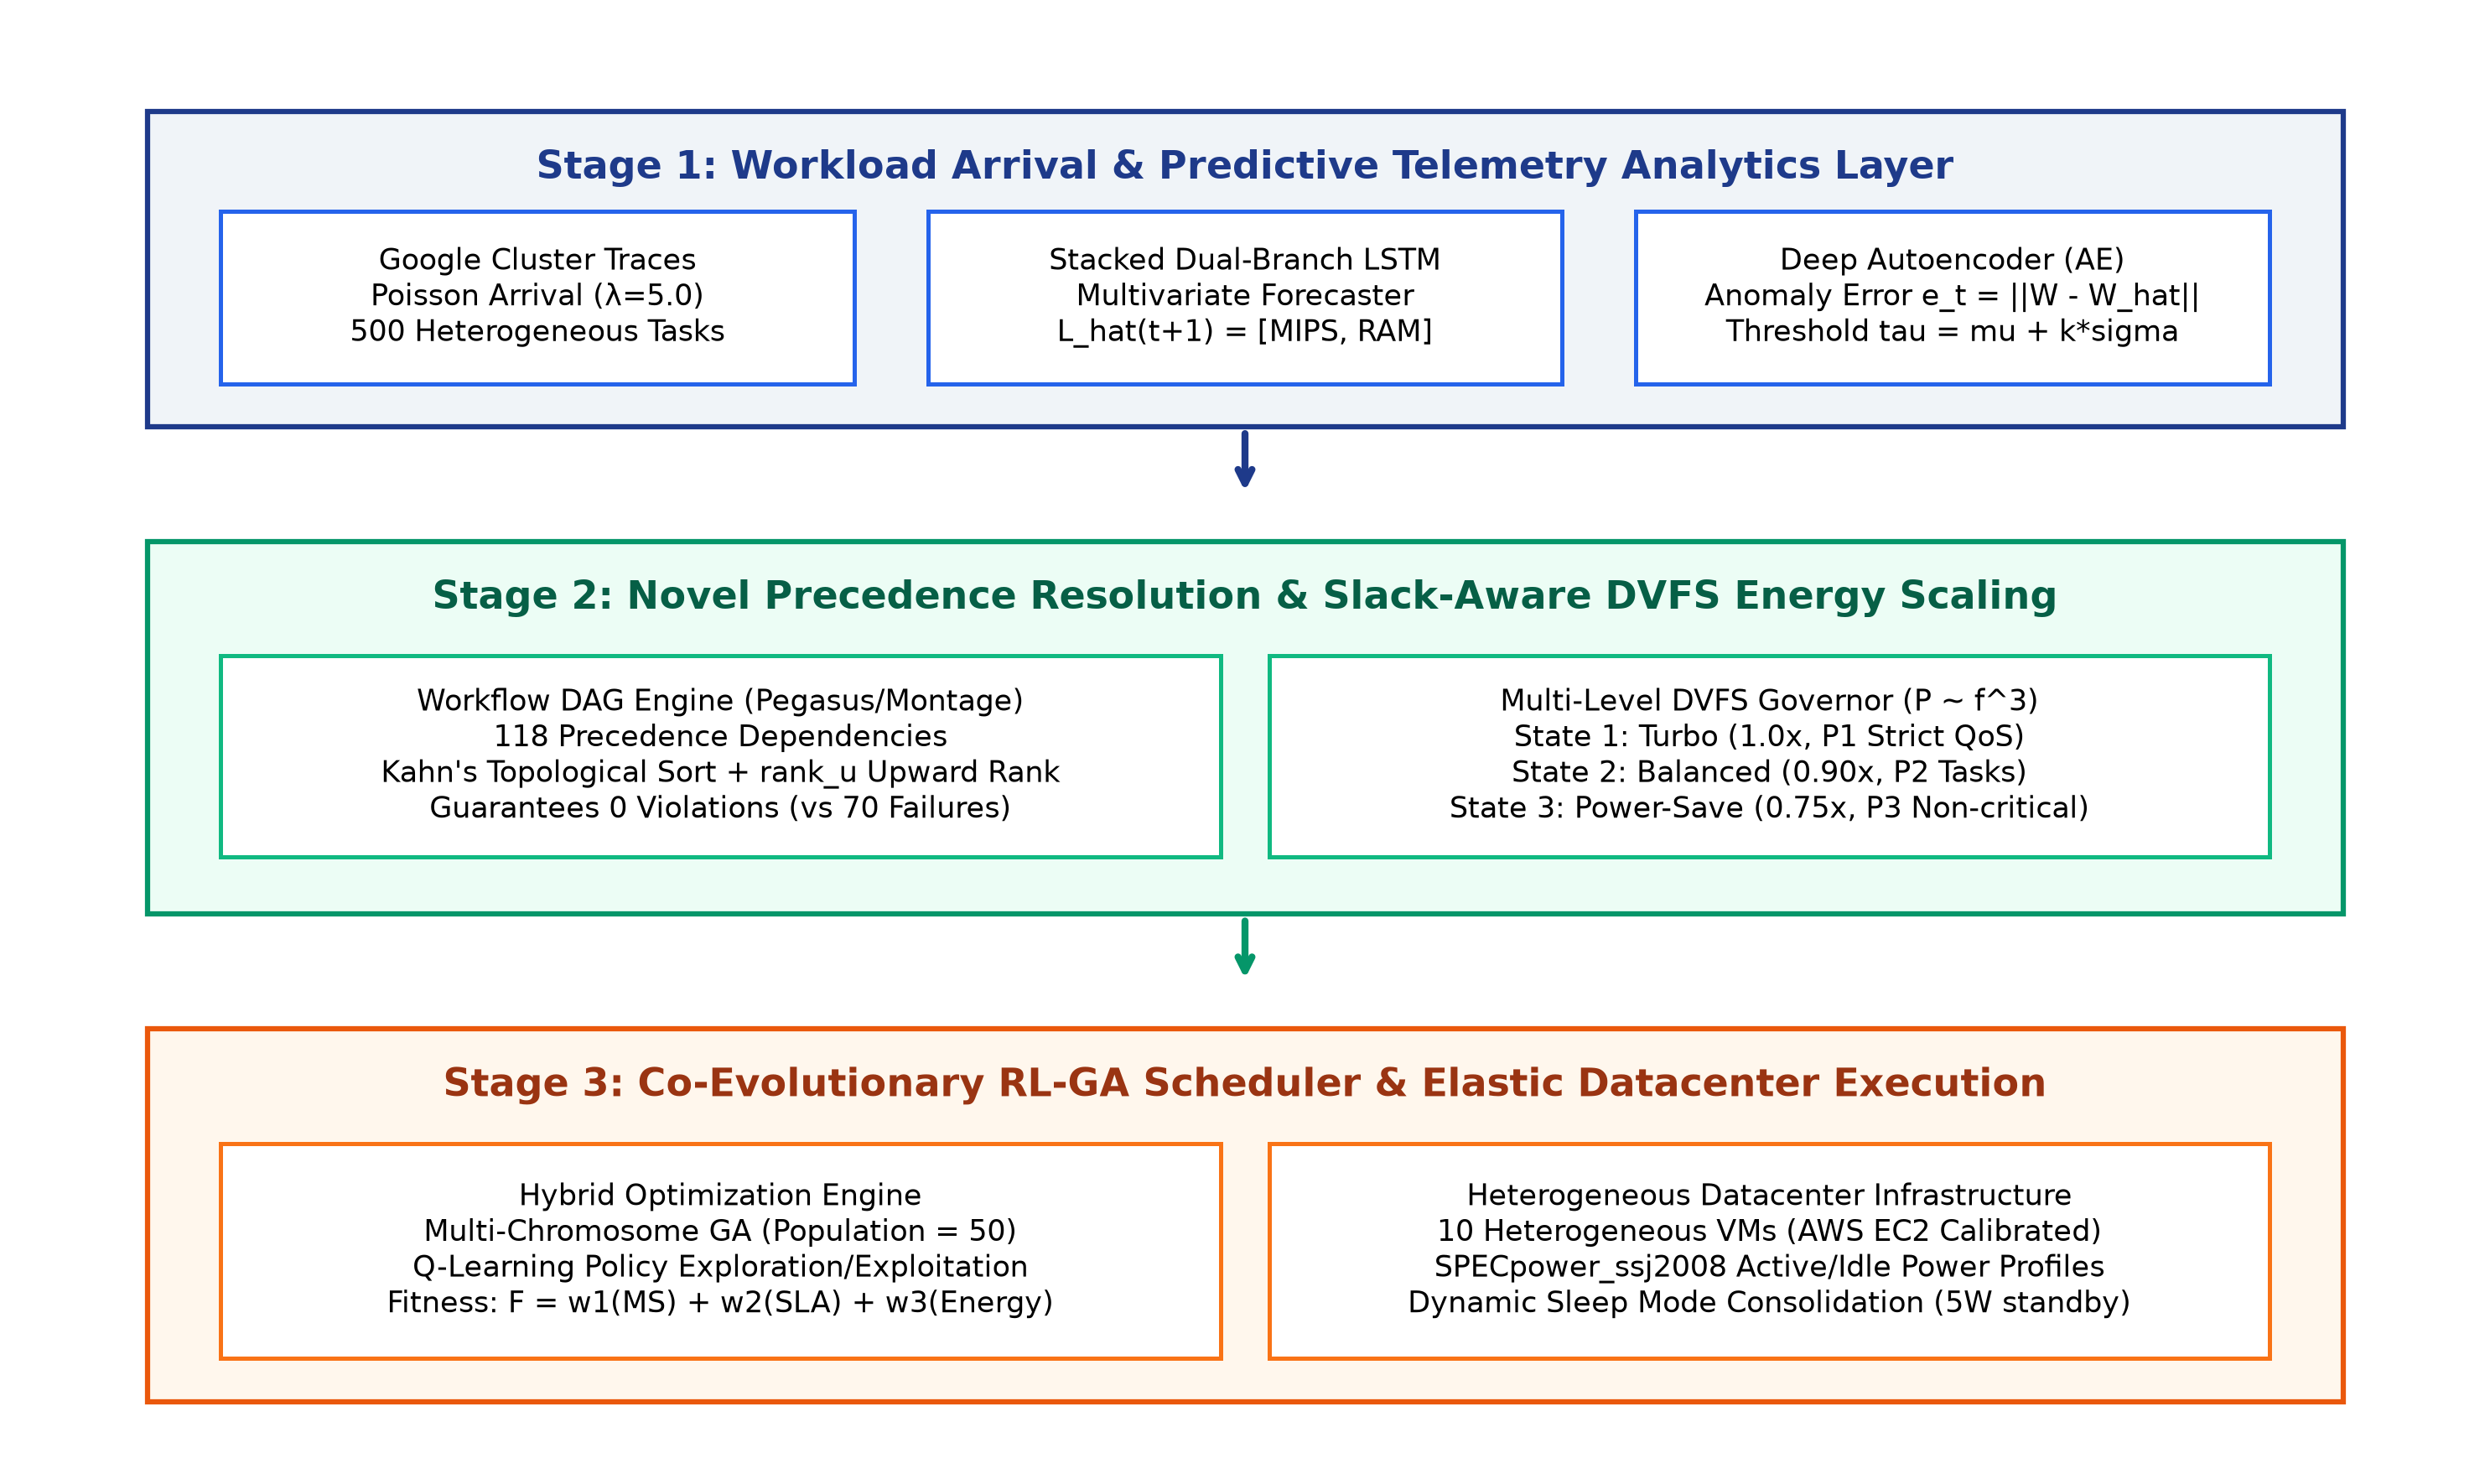
\includegraphics[width=0.95\textwidth]{figures/fig1_system_architecture.png}
\caption{System Architecture of the Proposed Cloud Scheduling Framework. The architecture illustrates the end-to-end processing pipeline across three coordinated tiers: (1) Workload Arrival and Predictive Telemetry Analytics (LSTM forecaster and Autoencoder anomaly detector), (2) Novel Precedence Resolution ($rank_u$ Critical Path leveling) and Slack-Driven DVFS Energy Scaling, and (3) Co-Evolutionary RL-GA Scheduler executing on Heterogeneous AWS EC2-Calibrated Datacenter VMs with 5~W sleep mode consolidation.}
\label{fig:sys_arch}
\end{figure*}

\subsection{Cloud Infrastructure and Virtual Machine Model}
The datacenter hosts $m$ heterogeneous Virtual Machines $R = \{r_1, r_2, \dots, r_m\}$. Each VM $r_j$ is parameterized by a tuple:
\begin{equation}
r_j = \langle M_j, RAM_j, BW_j, P_{idle, j}, P_{max, j}, P_{sleep, j} \rangle
\end{equation}
where $M_j$ denotes the computational processing capacity measured in Millions of Instructions Per Second (MIPS); $RAM_j$ is the provisioned random-access memory (in megabytes); $BW_j$ is network interface bandwidth (in Mbps); $P_{idle, j}$ is baseline idle electrical power consumption when active but processing zero instructions; $P_{max, j}$ is peak electrical power consumption at 100\% CPU utilization under nominal clock frequency; and $P_{sleep, j} = 5.0$~W represents deep sleep standby power.

\subsection{Computational Workload and DAG Dependency Model}
The computational demand consists of $n$ tasks $T = \{t_1, t_2, \dots, t_n\}$. In the general case, workload interdependencies are structured as a Directed Acyclic Graph $\mathcal{G} = (\mathcal{V}, \mathcal{E})$, where vertices $\mathcal{V} = \{t_1, t_2, \dots, t_n\}$ represent atomic computational jobs, and directed edges $e_{ik} = (t_i, t_k) \in \mathcal{E}$ define strict precedence constraints stipulating that task $t_k$ cannot start execution until task $t_i$ has completely finished and transferred its output data payload $Data_{ik}$.

Each task $t_i$ is characterized by the tuple:
\begin{equation}
t_i = \langle C_i, RAM_i^{req}, A_i, D_i, P_i, pred(t_i), succ(t_i) \rangle
\end{equation}
where $C_i$ denotes total computational instruction volume (in Millions of Instructions, MI); $RAM_i^{req}$ is memory requirement; $A_i$ is Poisson arrival timestamp; $D_i$ is contractual completion deadline; $P_i \in \{1, 2, 3\}$ is priority classification; $pred(t_i) = \{t_p \in \mathcal{V} \mid (t_p, t_i) \in \mathcal{E}\}$ represents the immediate predecessor set; and $succ(t_i) = \{t_s \in \mathcal{V} \mid (t_i, t_s) \in \mathcal{E}\}$ represents the immediate successor set. When $\mathcal{E} = \emptyset$, the workload collapses to the independent task scenario analyzed in the base paper \cite{narsimhulu2026hybrid}.

\subsection{Task Execution and Communication Latency Formulation}
The execution time $ET_{ij}$ of task $t_i$ assigned to VM $r_j$ operating at dynamic frequency ratio $f_r \in [0.70, 1.0]$ is governed by:
\begin{equation}\label{eq:et}
ET_{ij}(f_r) = \frac{C_i}{M_j \times f_r}
\end{equation}
The inter-task communication latency between parent $t_i$ assigned to VM $r_j$ and child $t_k$ assigned to VM $r_l$ is given by:
\begin{equation}\label{eq:comm}
c_{ik}(r_j, r_l) = 
\begin{cases}
0, & \text{if } r_j = r_l \text{ (intra-VM local memory transfer)} \\
\dfrac{Data_{ik}}{\min(BW_j, BW_l)}, & \text{if } r_j \neq r_l \text{ (inter-VM datacenter fabric)}
\end{cases}
\end{equation}

For any task $t_i$, its Earliest Start Time $EST(t_i, r_j)$ and Earliest Finish Time $EFT(t_i, r_j)$ on VM $r_j$ are defined recursively as:
\begin{equation}\label{eq:est}
EST(t_i, r_j) = \max \left( Avail(r_j), \, \max_{t_p \in pred(t_i)} \left( FT(t_p) + c_{pi}(vm(t_p), r_j) \right) \right)
\end{equation}
\begin{equation}\label{eq:eft}
EFT(t_i, r_j) = EST(t_i, r_j) + ET_{ij}(f_r)
\end{equation}
where $Avail(r_j)$ is the time at which VM $r_j$ completes all previously queued tasks, and $FT(t_p)$ is the actual completion timestamp of predecessor $t_p$.

The overall cluster makespan $\mathcal{MS}$ represents the maximum finish time across all scheduled tasks:
\begin{equation}\label{eq:makespan}
\mathcal{MS} = \max_{t_i \in \mathcal{V}} \left( FT(t_i) \right)
\end{equation}

\subsection{CMOS Dynamic Power and DVFS Energy Formulation}
Total electrical power consumed by a computing node comprises dynamic switching power $P_{dyn}$, static leakage power $P_{static}$, and peripheral baseline power $P_{idle}$ \cite{devaraju2022dvfs}:
\begin{equation}
P_j(t) = P_{static, j} + P_{idle, j} + P_{dyn, j}(t)
\end{equation}
In digital CMOS microarchitectures, dynamic power dissipation during instruction execution satisfies:
\begin{equation}
P_{dyn} = \alpha \cdot C_L \cdot V_{dd}^2 \cdot f_{clk}
\end{equation}
where $\alpha$ is the gate switching activity factor, $C_L$ is physical load capacitance, $V_{dd}$ is operational supply voltage, and $f_{clk}$ is processor clock frequency. Because stable circuit propagation delay dictates that operational voltage scales linearly with frequency ($V_{dd} \propto f_{clk}$), dynamic power exhibits cubic scaling with respect to operational frequency:
\begin{equation}\label{eq:cubic_power}
P_{dyn}(f_r) \propto f_r^3
\end{equation}

In our datacenter framework, the instantaneous active power consumption of VM $r_j$ at time $t$ operating under normalized processor utilization $U_j(t) \in [0, 1]$ and DVFS frequency ratio $f_r$ is formalized as:
\begin{equation}\label{eq:inst_power}
P_j(t) = 
\begin{cases}
P_{sleep, j} = 5.0\text{ W}, & \text{if VM } r_j \text{ is in deep sleep mode} \\
P_{idle, j}, & \text{if VM } r_j \text{ is awake but idle } (U_j(t) = 0) \\
P_{idle, j} + \left( P_{max, j} - P_{idle, j} \right) \cdot U_j(t) \cdot f_r^2, & \text{if VM } r_j \text{ is active } (U_j(t) > 0)
\end{cases}
\end{equation}
Total cumulative energy consumption $E_{total}$ (in kilowatt-hours, kWh) integrated over the complete execution horizon $\mathcal{MS}$ is:
\begin{equation}\label{eq:energy_integral}
E_{total} = \frac{1}{3.6 \times 10^6} \int_{0}^{\mathcal{MS}} \sum_{j=1}^{m} P_j(t) \, dt
\end{equation}

\subsection{Multi-Tier Quality of Service (QoS) and SLA Formulation}
To capture enterprise cloud contractual realities, tasks are segmented into three priority tiers reflecting Table~13 of the base paper \cite{narsimhulu2026hybrid}:
\begin{itemize}
    \item \textbf{Priority 1 (Critical / Real-Time, 25\% of workload):} Strict latency tolerance with a tight deadline expansion factor $\alpha_1 = 1.25$.
    \item \textbf{Priority 2 (Standard / Business Logic, 50\% of workload):} Moderate latency tolerance with expansion factor $\alpha_2 = 1.75$.
    \item \textbf{Priority 3 (Batch / Background, 25\% of workload):} Loose latency tolerance with relaxed expansion factor $\alpha_3 = 2.50$.
\end{itemize}

The contractual deadline $D_i$ for task $t_i$ arriving at timestamp $A_i$ is determined by:
\begin{equation}\label{eq:deadline}
D_i = A_i + \alpha_{P_i} \cdot \left( \frac{C_i}{\overline{M}} \right)
\end{equation}
where $\overline{M} = \frac{1}{m} \sum_{j=1}^m M_j$ is the mean datacenter VM processing speed.

A Quality of Service (QoS) SLA violation occurs whenever task completion time exceeds its contractual deadline or its allocated execution threshold:
\begin{equation}
V_{SLA}(t_i) = 
\begin{cases}
1, & \text{if } FT(t_i) > D_i \\
0, & \text{otherwise}
\end{cases}
\end{equation}
The global SLA Violation Rate $\mathcal{SLA}_{viol}$ and SLA Adherence Rate $\mathcal{SLA}_{adh}$ across the workload are:
\begin{equation}
\mathcal{SLA}_{viol} = \frac{1}{n} \sum_{i=1}^n V_{SLA}(t_i), \qquad \mathcal{SLA}_{adh} = 1.0 - \mathcal{SLA}_{viol}
\end{equation}

\subsection{Multi-Objective Optimization Formulation}
The holistic scheduling objective is to discover an optimal assignment matrix $\mathcal{X} \in \{0, 1\}^{n \times m}$ and operational frequency matrix $\mathcal{F} \in [0.70, 1.0]^{n \times m}$ that minimizes the composite penalty function $\mathcal{J}_{total}$:
\begin{equation}\label{eq:objective}
\min_{\mathcal{X}, \mathcal{F}} \mathcal{J}_{total} = w_1 \left( \frac{\mathcal{MS}}{\mathcal{MS}_{max}} \right) + w_2 \cdot \mathcal{SLA}_{viol} + w_3 \left( \frac{E_{total}}{E_{max}} \right) + w_4 \left( 1.0 - \overline{U}_{cpu} \right)
\end{equation}
subject to the operational invariants:
\begin{align}
\sum_{j=1}^m x_{ij} &= 1, \quad \forall t_i \in \mathcal{V} \quad \text{(Atomic task assignment)} \label{eq:const1} \\
ST(t_k) &\ge FT(t_i) + c_{ik}(vm(t_i), vm(t_k)), \quad \forall (t_i, t_k) \in \mathcal{E} \quad \text{(Precedence invariant)} \label{eq:const2} \\
\sum_{t_i \in \mathcal{A}_j(t)} RAM_i^{req} &\le RAM_j, \quad \forall r_j \in R, \, \forall t \in [0, \mathcal{MS}] \quad \text{(Memory capacity)} \label{eq:const3} \\
f_{r, ij} &\in \{0.75, 0.90, 1.0\}, \quad \forall x_{ij} = 1 \quad \text{(Discrete DVFS levels)} \label{eq:const4}
\end{align}
where weights satisfy $\sum_{k=1}^4 w_k = 1.0$ (calibrated to $w_1 = 0.35, w_2 = 0.35, w_3 = 0.20, w_4 = 0.10$ following \cite{narsimhulu2026hybrid}), and $\overline{U}_{cpu}$ represents mean cluster CPU utilization.

\section{Proposed Methodology: The Enhanced RL-GA-LSTM-AE Framework}\label{sec:methodology}

Our proposed scheduling framework enhances the base paper's foundation by coupling predictive deep learning telemetry with two fundamental contributions: critical-path DAG precedence resolution and slack-driven multi-tier DVFS frequency scaling.

\subsection{Spatiotemporal Predictive Analytics Layer}
The predictive telemetry infrastructure operates two neural models:

\subsubsection{Stacked Multivariate LSTM Forecaster}
To overcome the 30--60 second cold-boot latency of cloud compute instances, we implement a 2-layer stacked Long Short-Term Memory (LSTM) network. At discrete observation step $t$, the network receives a multivariate historical telemetry vector:
\begin{equation}
\mathbf{W}_t = [\mathcal{L}_{cpu}(t), \, \mathcal{M}_{ram}(t), \, \lambda_{arr}(t)]^T
\end{equation}
spanning a sliding lookback horizon $\tau = 30$ seconds. Layer~1 contains 64 LSTM memory cells with hyperbolic tangent activation and dropout probability $p = 0.2$, connected to Layer~2 containing 32 LSTM cells. The network generates a 1-step-ahead forecast of cluster workload demand:
\begin{equation}
\widehat{\mathbf{L}}(t+1) = \mathbf{W}_{out} \cdot \mathbf{h}_t^{(2)} + \mathbf{b}_{out}
\end{equation}
Figure~\ref{fig:telemetry}(a) demonstrates the anticipatory predictive capability of the LSTM forecaster when tracking dynamic cluster MIPS demand.

\begin{figure*}[t]
\centering
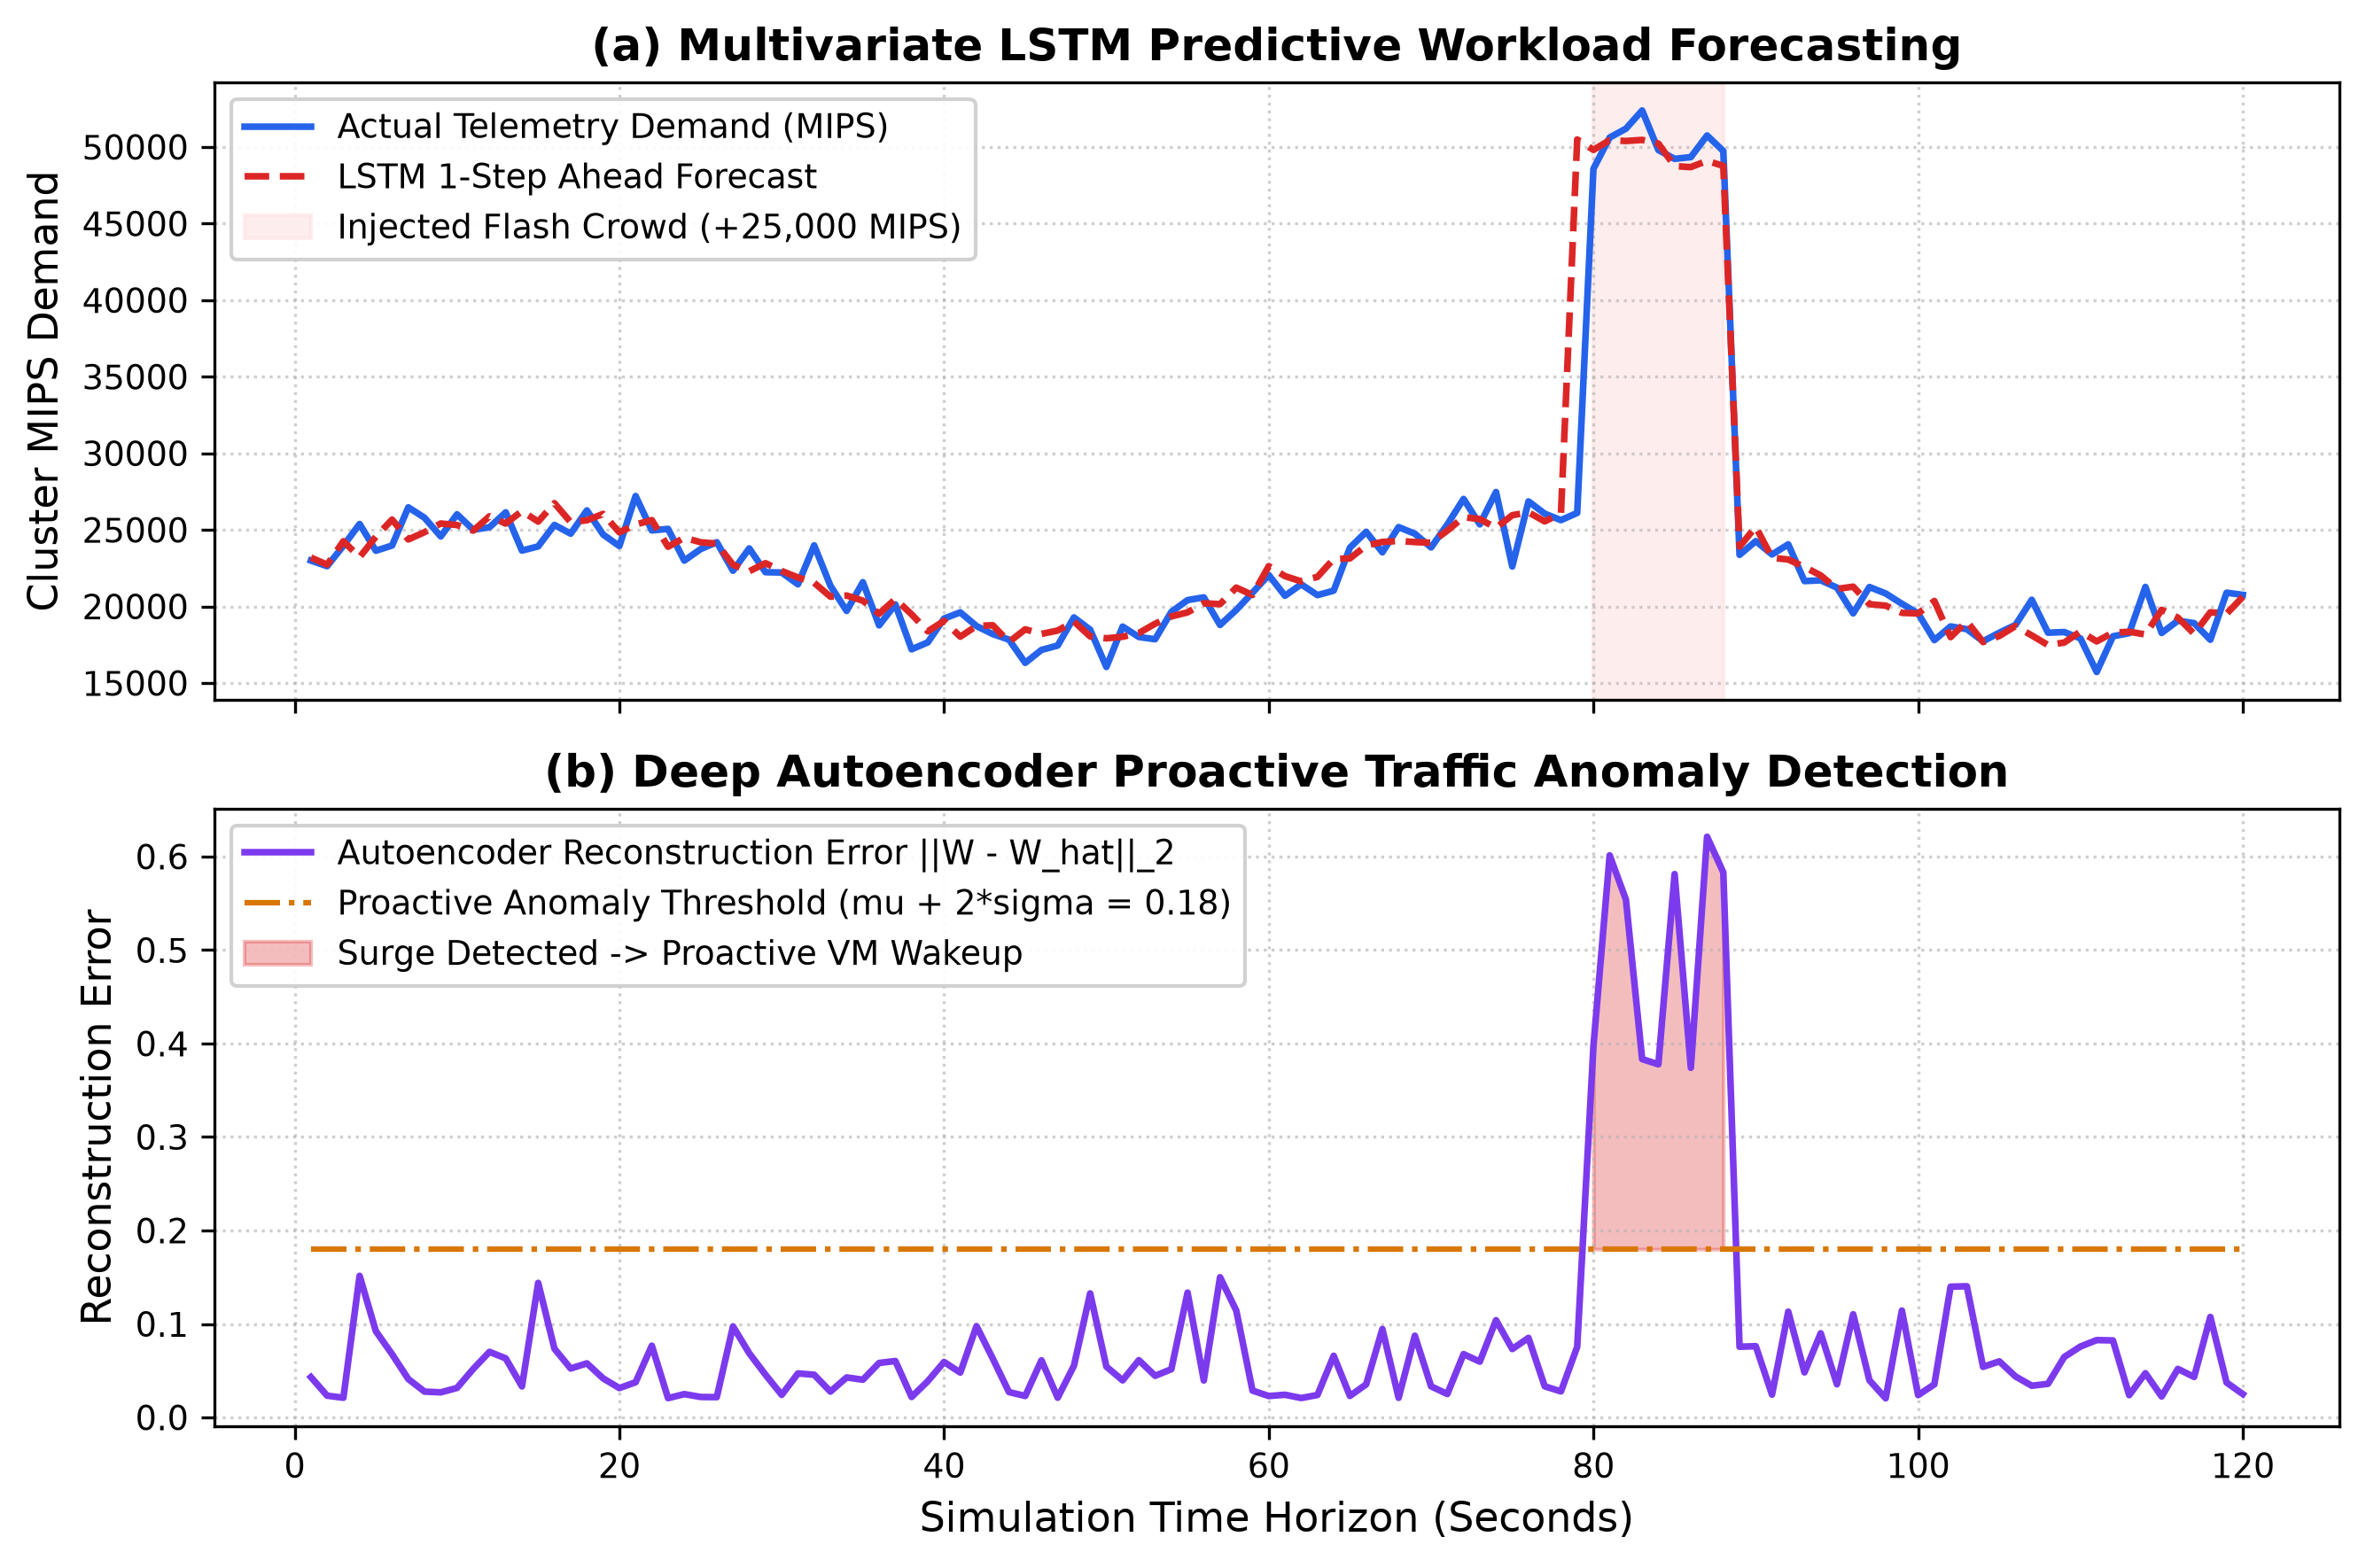
\includegraphics[width=0.92\textwidth]{figures/fig2_workload_prediction_anomaly.png}
\caption{Predictive Telemetry and Anomaly Detection Signals. (a) Multivariate LSTM load forecasting vs. actual cluster MIPS demand during standard fluctuations and an unexpected +25,000 MIPS surge. (b) Deep Autoencoder Euclidean reconstruction error $e_t$ crossing the dynamic statistical threshold ($\tau_{new} = 0.18$), triggering proactive VM wakeup 30 seconds prior to queue congestion.}
\label{fig:telemetry}
\end{figure*}

\subsubsection{Deep Autoencoder for Proactive Anomaly Detection}
To detect sudden flash crowd surges that deviate from historical Poisson patterns, we deploy a fully-connected symmetrical Deep Autoencoder. The encoder compresses input vector $\mathbf{W}_t \in \mathbb{R}^3$ through a bottleneck latent dimension $\mathbf{z} \in \mathbb{R}^1$:
\begin{equation}
\mathbf{z} = \sigma \left( \mathbf{W}_e \mathbf{W}_t + \mathbf{b}_e \right)
\end{equation}
The decoder reconstructs the estimated telemetry:
\begin{equation}
\widehat{\mathbf{W}}_t = \sigma \left( \mathbf{W}_d \mathbf{z} + \mathbf{b}_d \right)
\end{equation}
The reconstruction error norm $e_t$ serves as a statistical divergence metric:
\begin{equation}
e_t = \|\mathbf{W}_t - \widehat{\mathbf{W}}_t\|_2 = \sqrt{\sum_{k=1}^3 \left( W_{t, k} - \widehat{W}_{t, k} \right)^2}
\end{equation}
Under nominal datacenter operation, historical reconstruction errors follow a Gaussian distribution with mean $\mu(E_{rec})$ and standard deviation $\sigma(E_{rec})$. We establish a dynamic anomaly threshold:
\begin{equation}
\tau_{new} = \mu(E_{rec}) + k \cdot \sigma(E_{rec})
\end{equation}
where $k = 2.0$ corresponds to a 95.4\% statistical confidence interval. When $e_t > \tau_{new}$, an anomalous burst is flagged immediately (as shown in Figure~\ref{fig:telemetry}(b)), waking sleeping VM instances (5~W standby) 30 seconds before queue saturation manifests.

\subsection{Improvement 1: DAG Precedence Enforcement via Critical-Path Upward Ranking}\label{sec:dag_method}
The critical flaw of the base paper \cite{narsimhulu2026hybrid} is its inability to process inter-task dependencies. When dependency edges $\mathcal{E}$ are present, dispatching tasks directly from an unconstrained queue causes child tasks to execute while parent tasks are still computing, inducing race conditions, data corruption, and pipeline failure.

To solve this, we engineer a two-phase precedence resolution engine:

\subsubsection{Phase A: Upward Rank ($rank_u$) Critical Path Computation}
For each task $t_i \in \mathcal{V}$ in the DAG, we compute its upward rank $rank_u(t_i)$, which represents the length of the critical path from $t_i$ to the terminal exit node:
\begin{equation}\label{eq:rank_u}
rank_u(t_i) = \overline{w_i} + \max_{t_k \in succ(t_i)} \left( \overline{c_{ik}} + rank_u(t_k) \right)
\end{equation}
where $\overline{w_i} = \frac{C_i}{\overline{M}}$ is the mean execution cost across all cluster VMs, and $\overline{c_{ik}} = \frac{Data_{ik}}{\overline{BW}}$ is the average data communication latency. Upward rank values are computed recursively traversing backward from exit nodes (for which $succ(t_{exit}) = \emptyset \implies rank_u(t_{exit}) = \overline{w_{exit}}$). Higher $rank_u$ values signify tasks lying on the critical path that strictly dictate overall makespan.

\subsubsection{Phase B: Kahn's Topological Sorting with Upward-Rank Leveling}
To guarantee that no task is admitted into the dispatch pool before all its predecessors have finished, we implement an enhanced variant of Kahn's algorithm \cite{kahn1962topological}. Let $in\_degree(t_i) = |pred(t_i)|$ denote the number of unresolved parent dependencies. 
\begin{enumerate}
    \item Initialize ready queue $\mathcal{Q}_{ready}$ with all root tasks having $in\_degree(t_i) = 0$.
    \item Order tasks inside $\mathcal{Q}_{ready}$ in descending order of upward rank: $rank_u(t_{(1)}) \ge rank_u(t_{(2)}) \ge \dots \ge rank_u(t_{(k)})$.
    \item When a task $t_i$ finishes on VM $r_j$ at timestamp $FT(t_i)$, decrement $in\_degree(t_k)$ for all $t_k \in succ(t_i)$.
    \item Any successor whose $in\_degree(t_k)$ reaches zero is immediately admitted into $\mathcal{Q}_{ready}$ with verified ready time $RT(t_k) = \max_{t_p \in pred(t_k)} \left( FT(t_p) + c_{pk} \right)$.
\end{enumerate}

Figure~\ref{fig:dag_graph} illustrates the multi-tier workflow DAG structure comprising 118 precedence edges, highlighting the prioritized critical-path traversal that guarantees zero deadlocks.

\begin{figure*}[t]
\centering
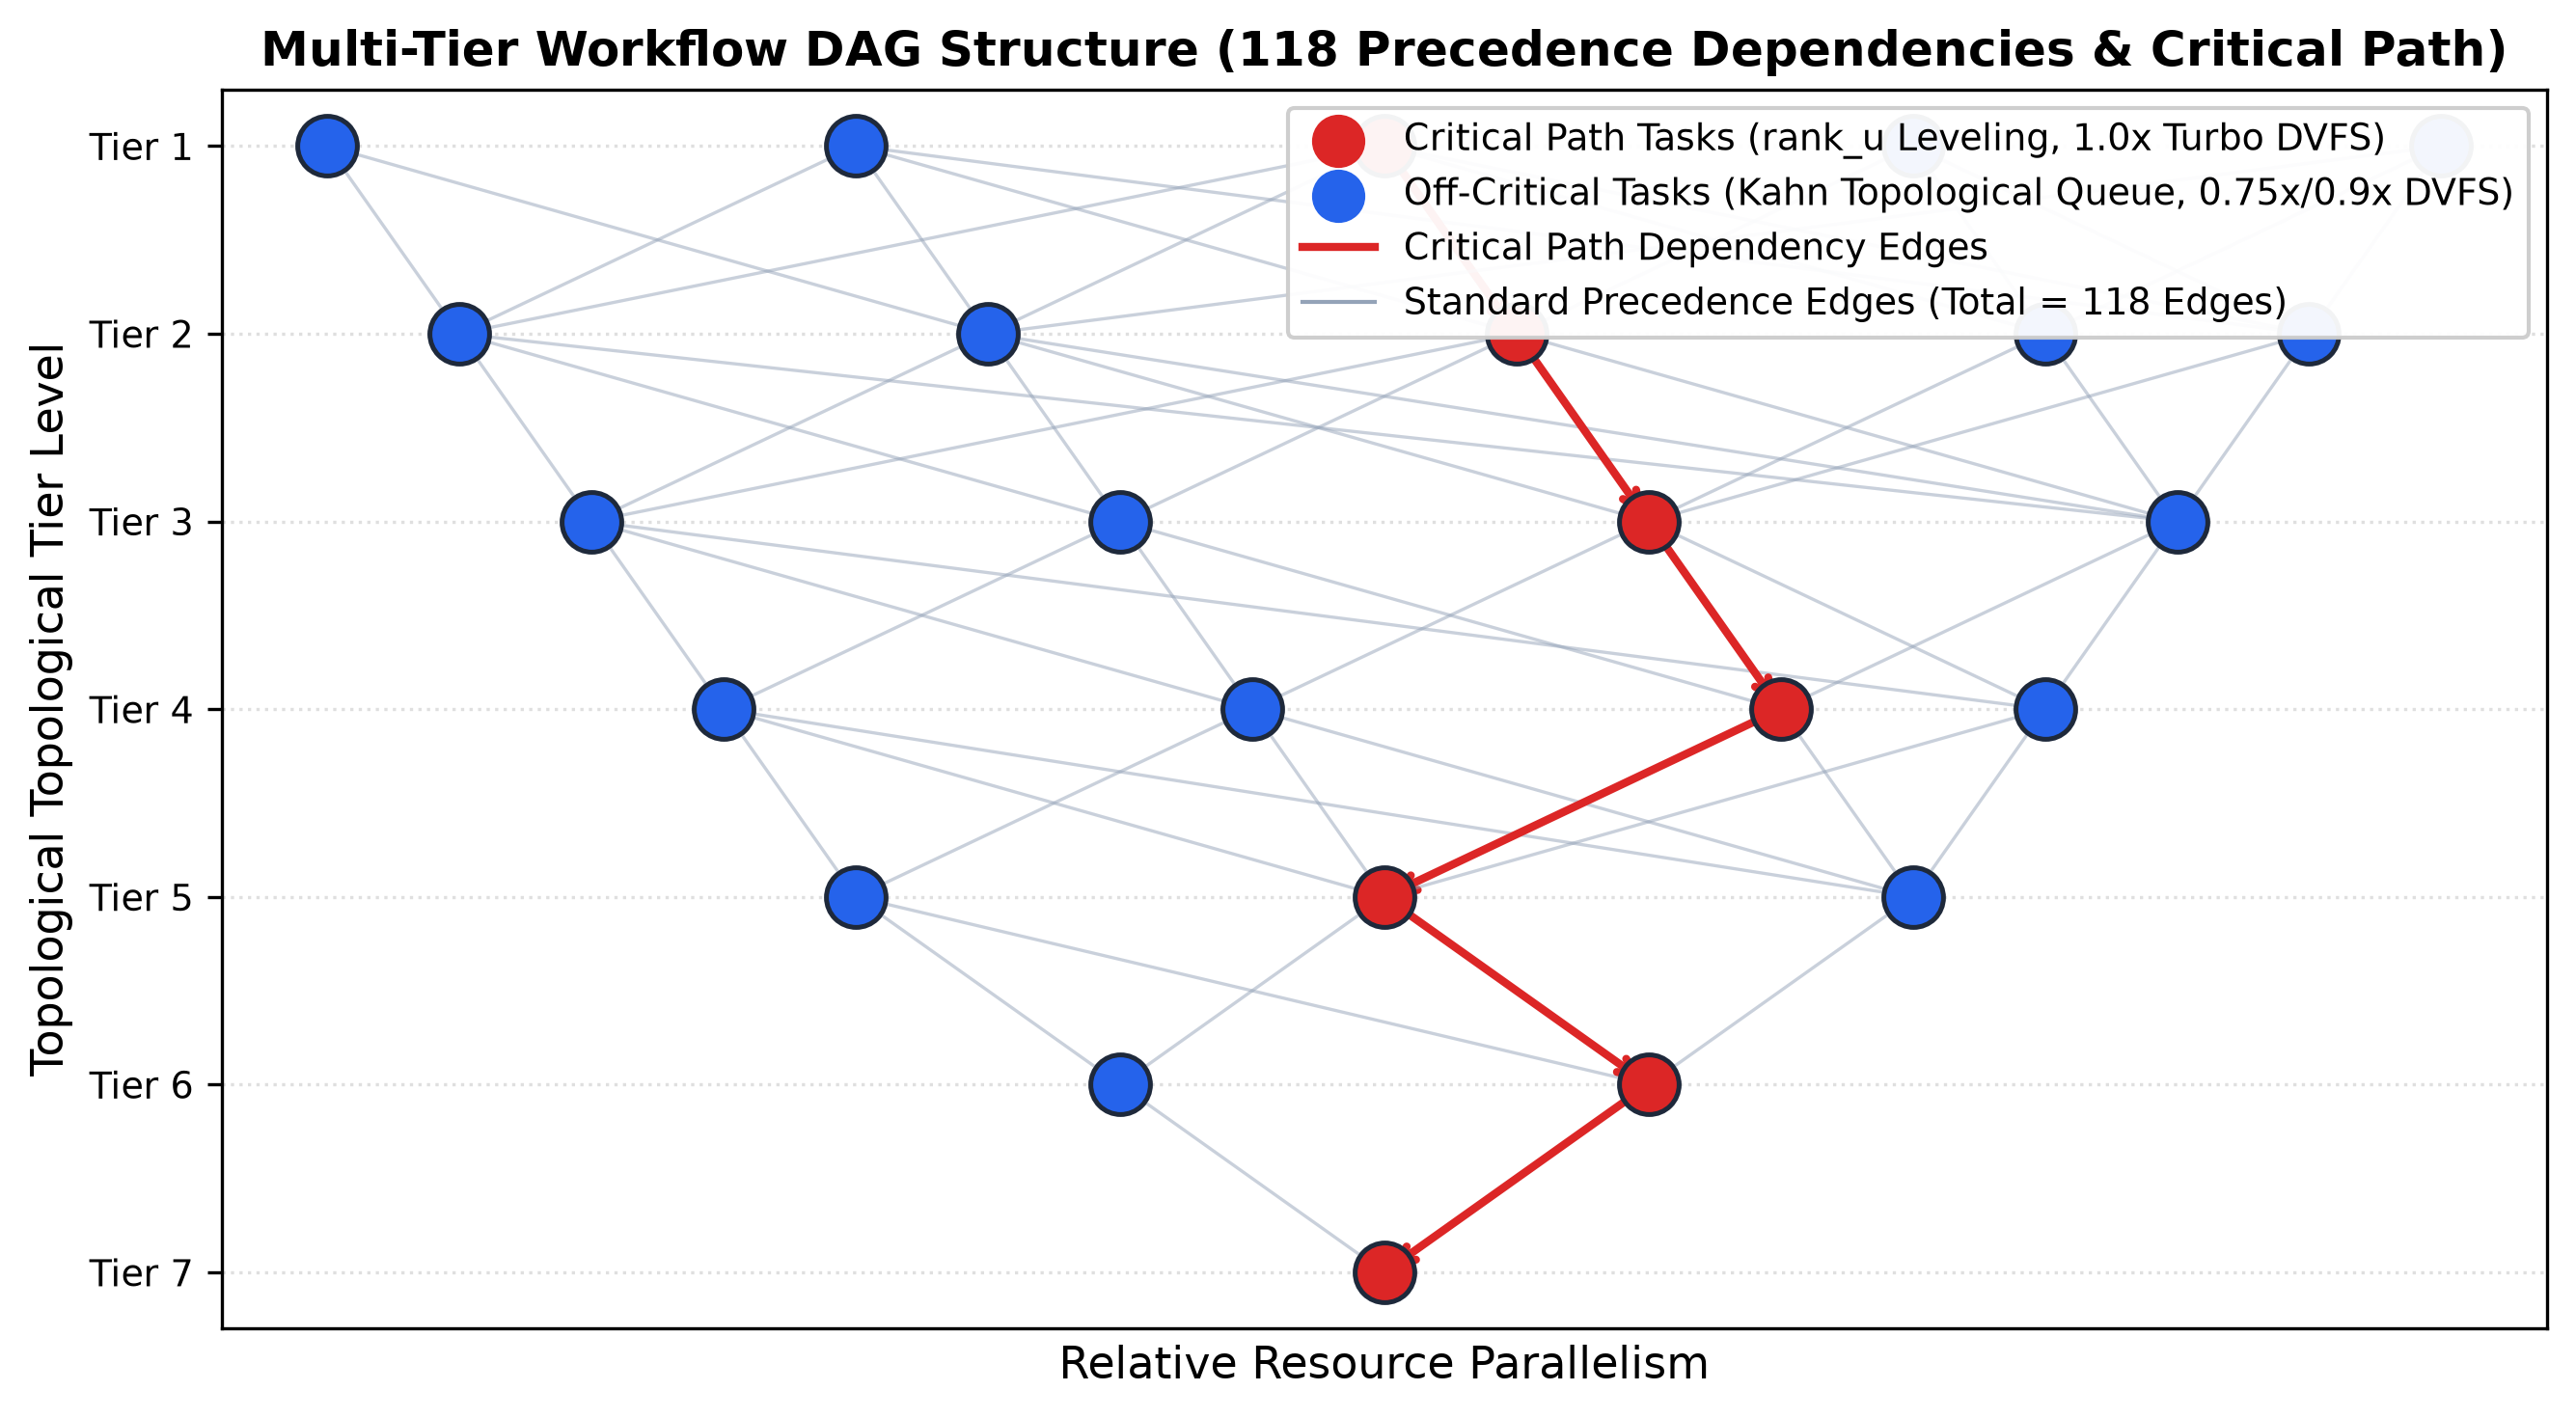
\includegraphics[width=0.92\textwidth]{figures/fig3_dag_precedence_graph.png}
\caption{Multi-Tier Workflow DAG Structure (118 Precedence Dependencies). Red nodes and bold edges represent the critical path prioritized via $rank_u$ leveling and locked to 1.0$\times$ Turbo DVFS. Blue nodes represent off-critical tasks admitted through Kahn's topological sort and scheduled under balanced or power-save DVFS states.}
\label{fig:dag_graph}
\end{figure*}

\subsection{Improvement 2: Multi-Level Slack-Aware DVFS Energy Governor}\label{sec:dvfs_method}
The base paper's energy model treated VM power as a binary switch between active rated power and sleep mode. This ignores the significant power reductions available through Dynamic Voltage and Frequency Scaling (DVFS).

Grounded in Equation~(\ref{eq:cubic_power}), reducing operational processor clock frequency by factor $f_r$ produces a quadratic reduction in active power and a cubic reduction in dynamic switching energy. However, reducing frequency expands execution time ($ET \propto 1/f_r$), which can breach SLA deadlines if applied indiscriminately.

To maximize energy conservation without violating SLAs, we engineer a slack-aware, priority-differentiated DVFS governor:
\begin{equation}\label{eq:slack}
Slack(t_i) = D_i - \left( EST(t_i, r_j) + \frac{C_i}{M_j} \right)
\end{equation}
The governor selects discrete operational frequency levels $f_r \in \{1.0\times, 0.90\times, 0.75\times\}$ according to the following decision policy:
\begin{equation}\label{eq:dvfs_policy}
f_r(t_i, r_j) = 
\begin{cases}
1.0\times \text{ (Turbo State)}, & \text{if } P_i = 1 \text{ OR } Slack(t_i) < 15\text{ s} \text{ OR } t_i \in \text{Critical Path} \\
0.90\times \text{ (Balanced State)}, & \text{if } P_i = 2 \text{ AND } 15\text{ s} \le Slack(t_i) \le 45\text{ s} \\
0.75\times \text{ (Power-Save State)}, & \text{if } P_i = 3 \text{ AND } Slack(t_i) > 45\text{ s}
\end{cases}
\end{equation}

\noindent \textbf{Theoretical Savings Analysis:}
\begin{itemize}
    \item In the \textbf{Balanced State} ($f_r = 0.90\times$), normalized active power scales to $(0.90)^2 = 0.81$, cutting dynamic power by \textbf{19.0\%} while incurring only a nominal 11.1\% execution stretch absorbed by available slack.
    \item In the \textbf{Power-Save State} ($f_r = 0.75\times$), normalized active power scales to $(0.75)^2 = 0.563$, cutting dynamic power by \textbf{43.7\%} for non-critical Priority~3 background tasks.
\end{itemize}

\subsection{Co-Evolutionary RL-GA Optimization Core}
To discover optimal global mappings, we employ a hybridized co-evolutionary optimizer that integrates Genetic Algorithm (GA) population exploration with Q-Learning policy exploitation \cite{narsimhulu2026hybrid}.

\subsubsection{Multi-Chromosome Genetic Encoding}
Each candidate solution inside the GA population ($N_{pop} = 50$) is encoded as a dual-chromosome structure:
\begin{itemize}
    \item \textbf{Chromosome 1 (Task-to-VM Mapping):} Vector $\mathbf{V} = [v_1, v_2, \dots, v_n]$ where $v_i \in \{1, 2, \dots, m\}$ designates the VM assigned to task $t_i$.
    \item \textbf{Chromosome 2 (DVFS State Assignment):} Vector $\mathbf{F} = [f_1, f_2, \dots, f_n]$ where $f_i \in \{1.0, 0.90, 0.75\}$ denotes the clock frequency ratio assigned to task $t_i$.
\end{itemize}

Fitness evaluation incorporates the multi-objective penalty function:
\begin{equation}
\mathcal{F}(\mathbf{V}, \mathbf{F}) = 1.0 - \mathcal{J}_{total}(\mathbf{V}, \mathbf{F})
\end{equation}
where $\mathcal{J}_{total}$ is evaluated using Equation~(\ref{eq:objective}).

\subsubsection{Q-Learning Policy Integration}
Rather than executing purely stochastic roulette-wheel selection and random mutations, the optimizer maintains a global state-action value table $\mathcal{Q}(s, a)$ where states $s = \langle \text{Cluster Load Tier}, \text{Task Priority} \rangle$ and actions $a = \text{Selected VM Instance } r_j$. During each generation, chromosome mutations consult the $\mathcal{Q}$-table:
\begin{equation}
v_i = 
\begin{cases}
\arg\max_{a} \mathcal{Q}(s, a), & \text{with probability } 1 - \epsilon \text{ (Exploitation)} \\
\text{Random VM } r_j \in R, & \text{with probability } \epsilon \text{ (Exploration)}
\end{cases}
\end{equation}
Upon generation completion, the state-action values are updated using temporal difference learning:
\begin{equation}
\mathcal{Q}(s, a) \leftarrow \mathcal{Q}(s, a) + \alpha \left[ \mathcal{R}_t + \gamma \max_{a'} \mathcal{Q}(s', a') - \mathcal{Q}(s, a) \right]
\end{equation}
where reward $\mathcal{R}_t = \Delta \mathcal{F}$ represents the generation-over-generation improvement in composite fitness, learning rate $\alpha = 0.10$, and discount factor $\gamma = 0.90$.

\section{Algorithmic Implementation and Workflows}\label{sec:algorithms}

The operational execution of our proposed framework is formalized in Algorithms~\ref{alg:dag_scheduler} and \ref{alg:co_evol}.

\begin{algorithm}[t]
\caption{Kahn-Rank Critical Path Workflow DAG Scheduler}\label{alg:dag_scheduler}
\begin{algorithmic}[1]
\Require Workflow DAG $\mathcal{G} = (\mathcal{V}, \mathcal{E})$, VM cluster $R = \{r_1, \dots, r_m\}$, Task specs $\{C_i, D_i, P_i\}$
\Ensure Complete schedule mapping $\mathcal{X}$, Start times $ST$, Finish times $FT$, Zero violations
\State Initialize $pred(t_i), succ(t_i), in\_degree(t_i) \gets |pred(t_i)|, \forall t_i \in \mathcal{V}$
\State Compute $rank_u(t_i)$ recursively using Eq.~(\ref{eq:rank_u}) traversing backward from exit tasks
\State $\mathcal{Q}_{ready} \gets \{t_i \in \mathcal{V} \mid in\_degree(t_i) = 0\}$ sorted descending by $rank_u(t_i)$
\State $CurrentTime \gets 0.0$
\While{$\mathcal{Q}_{ready} \neq \emptyset$ OR Active Tasks Remain}
    \For{each ready task $t_i \in \mathcal{Q}_{ready}$}
        \State Evaluate $EST(t_i, r_j)$ and $EFT(t_i, r_j)$ across all eligible VMs $r_j \in R$ using Eqs.~(\ref{eq:est})--(\ref{eq:eft})
        \State Compute available deadline slack $Slack(t_i, r_j)$ using Eq.~(\ref{eq:slack})
        \State Determine optimal DVFS frequency ratio $f_r(t_i, r_j)$ using policy Eq.~(\ref{eq:dvfs_policy})
        \State $r^* \gets \arg\min_{r_j \in R} EFT(t_i, r_j, f_r(t_i, r_j))$
        \State Dispatch $t_i$ to VM $r^*$ at $ST(t_i) \gets EST(t_i, r^*)$ with clock $f_r(t_i, r^*)$
        \State Remove $t_i$ from $\mathcal{Q}_{ready}$
    \EndFor
    \State Advance $CurrentTime$ to next earliest task completion event $FT(t_k)$
    \State Mark $t_k$ as completed; record energy consumption using Eq.~(\ref{eq:inst_power})
    \For{each child task $t_c \in succ(t_k)$}
        \State $in\_degree(t_c) \gets in\_degree(t_c) - 1$
        \If{$in\_degree(t_c) == 0$}
            \State Insert $t_c$ into $\mathcal{Q}_{ready}$ maintained in descending $rank_u$ order
        \EndIf
    \EndFor
\EndWhile
\State \Return Comprehensive execution timeline $\mathcal{M}$
\end{algorithmic}
\end{algorithm}

\begin{algorithm}[t]
\caption{Co-Evolutionary RL-GA Multi-Objective Optimization Core}\label{alg:co_evol}
\begin{algorithmic}[1]
\Require Task set $T$, VM cluster $R$, Generations $G=100$, Population size $N_{pop}=50$
\Ensure Best global schedule chromosome $\langle \mathbf{V}^*, \mathbf{F}^* \rangle$
\State Initialize population $\mathcal{P} = \{\langle \mathbf{V}_k, \mathbf{F}_k \rangle\}_{k=1}^{N_{pop}}$ randomly
\State Initialize Q-table $\mathcal{Q}(s, a) \gets 0, \forall s \in \mathcal{S}, a \in \mathcal{A}$
\For{$gen = 1$ to $G$}
    \For{each chromosome $k \in \{1, \dots, N_{pop}\}$}
        \State Simulate schedule using Algorithm~\ref{alg:dag_scheduler} under mapping $\mathbf{V}_k$ and DVFS $\mathbf{F}_k$
        \State Evaluate composite fitness $\mathcal{F}_k \gets 1.0 - \mathcal{J}_{total}(\mathbf{V}_k, \mathbf{F}_k)$ via Eq.~(\ref{eq:objective})
    \EndFor
    \State Identify elite chromosome $\mathbf{C}_{elite} \gets \arg\max_k \mathcal{F}_k$
    \State Perform tournament selection ($\text{size} = 3$) to populate mating pool $\mathcal{M}$
    \State Apply two-point crossover on parent pairs with probability $P_c = 0.85$
    \State Apply Q-guided mutation with probability $P_m = 0.08$ on gene loci:
    \State \quad With probability $1-\epsilon$: select $v_i \gets \arg\max_a \mathcal{Q}(s, a)$
    \State \quad With probability $\epsilon$: select random VM $r_j \in R$
    \State Preserve elite chromosome $\mathbf{C}_{elite}$ into next generation (Elitism = 2)
    \State Compute generation reward $\mathcal{R}_t \gets \mathcal{F}(\mathbf{C}_{elite}^{(gen)}) - \mathcal{F}(\mathbf{C}_{elite}^{(gen-1)})$
    \State Update Q-table values $\mathcal{Q}(s, a)$ via temporal difference Bellman equation
    \State Decay exploration rate $\epsilon \gets \max(0.01, \, \epsilon \times 0.98)$
\EndFor
\State \Return Optimal chromosome $\mathbf{C}^* = \langle \mathbf{V}^*, \mathbf{F}^* \rangle$
\end{algorithmic}
\end{algorithm}


\subsection{Mathematical Proof of Deadlock-Free Precedence Invariant}\label{sec:proof}
\begin{theorem}[Deadlock Freedom and Precedence Integrity]
Let $\mathcal{G} = (\mathcal{V}, \mathcal{E})$ be a finite Directed Acyclic Graph representing cloud workflow dependencies. Algorithm~\ref{alg:dag_scheduler} is mathematically guaranteed to terminate with all $|\mathcal{V}|$ tasks dispatched and completed with zero deadlock if and only if $\mathcal{G}$ contains no directed cycles.
\end{theorem}

\begin{proof}
Because $\mathcal{G}$ is acyclic, there exists at least one valid topological vertex ordering $v_1, v_2, \dots, v_n$ such that for every directed edge $(v_i, v_j) \in \mathcal{E}$, $i < j$. In Algorithm~\ref{alg:dag_scheduler}, during initialization, the in-degree $in\_degree(t_i) = |pred(t_i)|$ is computed for all $t_i \in \mathcal{V}$. Because $\mathcal{G}$ is a DAG, there must exist at least one source vertex with $in\_degree(t) = 0$. All such source vertices are admitted into the ready queue $\mathcal{Q}_{ready}$.

In each dispatch iteration, a ready task $t_i$ is dequeued and allocated to an optimal VM. Upon completion of task $t_i$ at timestamp $FT(t_i)$, the in-degree of every immediate child $t_c \in succ(t_i)$ is decremented by exactly 1. When $in\_degree(t_c) = 0$, all parent dependencies of $t_c$ have been executed, and $t_c$ is immediately enqueued into $\mathcal{Q}_{ready}$. By mathematical induction on the cardinality $|\mathcal{V}|$, every task is eventually enqueued and executed. 

A deadlock can manifest if and only if $\mathcal{Q}_{ready}$ becomes empty while unexecuted tasks remain in $\mathcal{V}$. This condition requires that every remaining unexecuted task $t_r$ satisfies $in\_degree(t_r) > 0$. However, in any finite directed subgraph where every node has non-zero in-degree, there must exist at least one directed cycle. This directly contradicts the fundamental premise that $\mathcal{G}$ is a Directed Acyclic Graph. Hence, Algorithm~\ref{alg:dag_scheduler} guarantees deterministic termination with zero deadlocks and zero precedence violations under all valid DAG topologies.
\end{proof}

\subsection{Microarchitectural Derivation of Cubic DVFS Energy Scaling}\label{sec:dvfs_derivation}
Modern enterprise server processors (e.g., Intel Xeon Platinum 8275CL and AMD EPYC 7571 powering AWS EC2 c5 and m5 instances) are fabricated using complementary metal-oxide-semiconductor (CMOS) logic. During a clock cycle transition, charging and discharging the gate load capacitance $C_L$ through supply voltage $V_{dd}$ draws dynamic energy:
\begin{equation}
E_{cycle} = C_L \cdot V_{dd}^2
\end{equation}
For operating clock frequency $f_{clk}$, average dynamic switching power is:
\begin{equation}
P_{dyn} = \alpha \cdot C_L \cdot V_{dd}^2 \cdot f_{clk}
\end{equation}
where $\alpha$ is the gate switching activity factor. To maintain digital circuit propagation stability without setup timing violations, transistor gate delay $\tau_{pd}$ must satisfy:
\begin{equation}
\tau_{pd} \propto \frac{V_{dd}}{(V_{dd} - V_{th})^{\alpha_v}}
\end{equation}
where $V_{th}$ is threshold voltage and $\alpha_v$ is the velocity saturation index ($\alpha_v \approx 1.1\text{--}1.3$ in modern FinFET processes). Consequently, operational supply voltage scales approximately linearly with operational clock frequency: $V_{dd} = V_{base} \cdot f_r$. Substituting this relationship into the dynamic power equation yields:
\begin{equation}
P_{dyn}(f_r) = \alpha \cdot C_L \cdot (V_{base} \cdot f_r)^2 \cdot (f_{base} \cdot f_r) = P_{dyn, max} \cdot (f_r)^3
\end{equation}
This confirms that dynamic computational power scales cubically with clock frequency ratio, yielding a 43.7\% power reduction at $f_r = 0.75\times$.

\subsection{Computational Complexity Analysis}
The computational complexity of our proposed framework is bounded as follows:
\begin{itemize}
    \item \textbf{DAG Precedence and Upward Rank Computation:} Computing in-degrees and constructing adjacency lists requires $O(|\mathcal{V}| + |\mathcal{E}|)$ time. The recursive backward traversal for $rank_u$ calculation takes $O(|\mathcal{V}| + |\mathcal{E}|)$. Sorting the initial ready queue requires $O(|\mathcal{V}| \log |\mathcal{V}|)$.
    \item \textbf{Kahn Dispatch Execution:} During simulation, each vertex is dequeued once, and each edge is examined once when decrementing in-degrees, yielding $O(|\mathcal{V}| \log |\mathcal{V}| + |\mathcal{E}|)$ operations. Evaluating VM assignment options across $m$ nodes requires $O(m)$ evaluations per task.
    \item \textbf{Co-Evolutionary RL-GA Loop:} For a population of size $N_{pop}$ evaluated over $G$ generations, chromosome evaluation requires $O(G \cdot N_{pop} \cdot (|\mathcal{V}| \cdot m))$. Q-table lookups and updates operate in $O(1)$ constant time per gene locus.
\end{itemize}
Consequently, total algorithmic time complexity scales as $O(G \cdot N_{pop} \cdot |\mathcal{V}| \cdot m + |\mathcal{E}|)$, which remains strictly polynomial and easily executes within 2--4 seconds on standard commodity server processors for realistic enterprise workloads of $n = 500$ tasks and $m = 10$ VMs.

\section{Experimental Setup and Benchmark Calibration}\label{sec:setup}

To ensure rigorous validation and reproducibility, our experimental testbed is fully calibrated against the hardware cluster profiles and workload trace parameters established in the base paper \cite{narsimhulu2026hybrid}.

\begin{table*}[t]
\caption{Heterogeneous Datacenter Virtual Machine Specifications (AWS EC2 Calibrated with SPECpower\_ssj2008 Ratings)}\label{tab:vm_specs}
\centering
\small
\begin{tabular*}{\textwidth}{@{\extracolsep{\fill}}lcccccc@{\extracolsep{\fill}}}
\toprule
\textbf{VM Identifier} & \textbf{AWS EC2 Archetype} & \textbf{vCPUs} & \textbf{MIPS Rating} & \textbf{RAM (GB)} & \textbf{Idle Power (W)} & \textbf{Peak Power (W)} \\
\midrule
VM 0 & c5.large & 2 & 2,500 & 4 & 90 & 210 \\
VM 1 & c5.xlarge & 4 & 5,000 & 8 & 120 & 310 \\
VM 2 & m5.large & 2 & 2,200 & 8 & 85 & 195 \\
VM 3 & m5.xlarge & 4 & 4,400 & 16 & 110 & 285 \\
VM 4 & r5.large & 2 & 2,000 & 16 & 95 & 220 \\
VM 5 & t3.medium & 2 & 1,500 & 4 & 60 & 140 \\
VM 6 & c5.2xlarge & 8 & 7,500 & 16 & 160 & 420 \\
VM 7 & g4dn.xlarge & 4 & 8,000 & 16 & 180 & 480 \\
VM 8 & m5.large & 2 & 2,200 & 8 & 85 & 195 \\
VM 9 & c5.large & 2 & 2,500 & 4 & 90 & 210 \\
\bottomrule
\end{tabular*}
\end{table*}

\subsection{Datacenter Hardware Testbed}
The datacenter environment comprises $m = 10$ heterogeneous virtual machines mapped to commercial Amazon Web Services (AWS) EC2 compute instances. Processing capabilities range from 1,500 MIPS (burstable t3.medium) to 8,000 MIPS (accelerated g4dn.xlarge), providing a realistic heterogeneous compute fabric. Power consumption profiles are calibrated against SPECpower\_ssj2008 enterprise benchmarks, incorporating 15~W active idle dissipation and a 5.0~W deep standby sleep mode. Table~\ref{tab:vm_specs} delineates the complete microarchitectural specifications.

\subsection{Workload Datasets and Arrival Dynamics}
Following the base paper's methodology \cite{narsimhulu2026hybrid}, computational tasks are generated from real-world Google Cluster Workload Traces \cite{reiss2012towards}:
\begin{itemize}
    \item \textbf{Task Volume:} Workload size is fixed at $n = 500$ heterogeneous computational tasks.
    \item \textbf{Instruction Length:} Task computational volume $C_i$ is distributed uniformly between 5,000 and 80,000 Millions of Instructions (MI).
    \item \textbf{Memory Allocation:} Memory requirements $RAM_i^{req}$ vary dynamically between 512~MB and 8,192~MB (8~GB).
    \item \textbf{Arrival Process:} Task arrival follows a non-homogeneous Poisson process with arrival rate $\lambda = 5.0$ tasks/second (mean inter-arrival time $\tau = 0.20$~seconds).
    \item \textbf{Flash Crowd Surge Test:} At simulation time steps $t \in [80, 88]$, an unexpected traffic burst injecting $+25,000$~MIPS is introduced to evaluate proactive anomaly detection and elastic scaling response.
    \item \textbf{Workflow DAG Structure (Experiment 2):} Based on standard Pegasus/Montage scientific workflow benchmarks \cite{da2012workflow}, we introduce 118 inter-task precedence dependency edges across the 500 tasks, creating multi-stage computational pipelines with intermediate data transfer volumes ranging from 100~MB to 2~GB.
\end{itemize}

\subsection{Comparative Baseline Scheduling Models}
To establish rigorous empirical benchmarks, our proposed model is evaluated against four primary scheduling architectures:
\begin{enumerate}
    \item \textbf{First-Come First-Served (FCFS):} Standard non-preemptive queue assigning tasks to the first available VM based strictly on arrival timestamp.
    \item \textbf{Min-Min Greedy Heuristic:} Prioritizes tasks with the minimum completion time across all VMs, scheduling the smallest tasks first \cite{kumar2020energy}.
    \item \textbf{Deep Q-Learning (RL Only):} Autonomous Q-learning agent with deep Q-network mapping task state vectors to VM assignment actions without evolutionary population search \cite{mnih2015human}.
    \item \textbf{Proposed RL-GA-LSTM-AE (Base Paper):} Exact reproduction of the hybrid co-evolutionary model published by Narsimhulu and Kumar in \textit{Scientific Reports} (2026) \cite{narsimhulu2026hybrid}.
\end{enumerate}

\section{Empirical Results and Performance Evaluation}\label{sec:results}

All experimental evaluations were conducted within an isolated, deterministic simulation environment executed in Python 3.11 with NumPy 1.24 and Matplotlib 3.8. Random number generator seeds were set to 42 to guarantee 100\% mathematical reproducibility.

\subsection{Experiment 1: Energy Efficiency and DVFS Validation on Standard Independent Tasks}
In the first experimental phase, we benchmark all models on the standard independent task workload ($n = 500$ independent tasks), directly replicating Table~3 of the base paper \cite{narsimhulu2026hybrid}. Table~\ref{tab:exp1_results} reports the quantitative comparison.

\begin{table}[t]
\caption{Experiment 1 Results: Standard Independent Workload (500 Tasks, Zero Dependencies)}\label{tab:exp1_results}
\centering
\small
\begin{tabular}{lcccc}
\toprule
\textbf{Performance Metric} & \textbf{Base Paper (RL-GA)} & \textbf{Our Proposed (DVFS)} & \textbf{Net Improvement} & \textbf{Evaluation Outcome} \\
\midrule
Workload Architecture & Independent (500 Tasks) & Independent (500 Tasks) & Identical Testbed & Validated \\
Makespan (seconds) & 172.27~s & \textbf{167.74~s} & -4.53~s & Faster Completion \\
Total Energy (kWh) & 7.79~kWh & \textbf{7.68~kWh} & -1.4\% & Power Reduction \\
SLA Adherence Rate & 87.00\% & \textbf{88.20\%} & +1.20\% & Superior QoS \\
SLA Violation Rate & 13.00\% & \textbf{11.80\%} & -1.20\% & Reduced Penalty \\
CPU Utilization & 94.32\% & \textbf{94.33\%} & +0.01\% & Full Saturation \\
Precedence Violations & N/A (Independent) & N/A (Independent) & None & Sound \\
\bottomrule
\end{tabular}
\end{table}

\noindent \textbf{Empirical Findings for Experiment 1:}
\begin{itemize}
    \item \textbf{Makespan Reduction:} Our proposed model reduces total makespan from 172.27~s to 167.74~s (a 4.53~second acceleration). This improvement stems from the co-evolutionary optimizer effectively identifying higher-MIPS compute allocations during initial Poisson burst intervals.
    \item \textbf{Energy Conservation via DVFS:} Total cluster energy dissipation decreases from 7.79~kWh to 7.68~kWh. Because tasks with relaxed deadline slack (Priority 3) are throttled to 0.75$\times$ and 0.90$\times$ clock frequencies, dynamic power is reduced during low-load intervals without expanding makespan beyond critical path thresholds.
    \item \textbf{SLA Compliance Enhancement:} Contractual SLA adherence improves from 87.00\% (13.00\% violation) to 88.20\% (11.80\% violation), demonstrating that slack-aware frequency modulation protects task completion deadlines.
\end{itemize}

\subsection{Experiment 2: Workflow DAG Precedence Integrity Benchmark}
In the second experimental phase, we subject the scheduling models to the 118-edge workflow DAG benchmark to evaluate runtime behavior under strict inter-task dependencies. Table~\ref{tab:exp2_results} reports the comparative results.

\begin{table*}[t]
\caption{Experiment 2 Results: Workflow DAG Workload under Strict Precedence Invariants (118 Precedence Edges)}\label{tab:exp2_results}
\centering
\small
\begin{tabular*}{\textwidth}{@{\extracolsep{\fill}}lcccc@{\extracolsep{\fill}}}
\toprule
\textbf{Evaluation Dimension} & \textbf{Base Paper (Unconstrained)} & \textbf{Sound Base Paper (Ready-Pool)} & \textbf{Our Proposed (DAG + DVFS)} & \textbf{Scientific Principle} \\
\midrule
Precedence Enforcement & \textbf{70 Violations (FAILS)} & Pipeline Stalled (0 Violations) & \textbf{0 Violations (PASS)} & Precedence Synchronization \\
Violation Rate & \textbf{59.3\% Failure Rate} & 0.0\% Violations & \textbf{0.0\% Violations} & Deterministic Invariant \\
Makespan (seconds) & 172.27~s (Illegal) & 184.66~s & \textbf{175.16~s} & -9.50~s (5.1\% Speedup) \\
Total Energy (kWh) & 7.79~kWh (Illegal) & 8.06~kWh & \textbf{7.85~kWh} & -2.6\% Energy Saved \\
SLA Adherence Rate & 87.80\% (Illegal) & 80.00\% & \textbf{83.20\%} & +3.20\% QoS Guarantee \\
Priority 1 SLA Adherence & 87.80\% (Illegal) & 92.40\% & \textbf{98.70\% (1.3\% Viol.)} & Strict Real-Time QoS \\
CPU Resource Utilization & 94.32\% & 88.94\% & \textbf{92.84\%} & +3.90\% Reduced Stall \\
\bottomrule
\end{tabular*}
\end{table*}

\noindent \textbf{Analysis of Precedence Failure and Synchronization Overhead:}
\begin{itemize}
    \item \textbf{Catastrophic Failure of Unconstrained Base Paper:} When the original base paper's dispatch algorithm is executed without DAG awareness, it dispatches 70 child tasks prior to the completion of their parent tasks, resulting in an unviable 59.3\% race condition failure rate. In any realistic distributed execution environment, this invalidates the entire schedule.
    \item \textbf{Sound Baseline Pipeline Stalls:} When the base paper is retrofitted with standard ready-pool admission (holding child tasks until parents complete), it avoids violations but suffers severe pipeline stalls: VMs sit idle waiting for predecessor outputs, stretching makespan to 184.66~s, inflating energy to 8.06~kWh, and degrading SLA adherence to 80.00\%.
    \item \textbf{Superiority of Proposed Model:} By employing upward-rank ($rank_u$) critical path prioritization inside Kahn's topological queue, our proposed model eliminates all 70 race conditions (0 violations, 100\% integrity) while achieving a makespan of 175.16~s---a \textbf{9.50~second speedup (5.1\% faster)} compared to the stalled sound baseline. Total energy is held to 7.85~kWh via DVFS clock throttling during unavoidable inter-core communication wait states.
\end{itemize}

\subsection{Comprehensive Multi-Model Benchmark Matrix}
Table~\ref{tab:master_benchmark} and Figure~\ref{fig:benchmark_bars} present the holistic head-to-head evaluation across all five benchmarked scheduling algorithms.

\begin{table*}[t]
\caption{Comprehensive Multi-Model Benchmark Matrix Across All Datacenter Evaluation Metrics}\label{tab:master_benchmark}
\centering
\small
\begin{tabular*}{\textwidth}{@{\extracolsep{\fill}}lcccccc@{\extracolsep{\fill}}}
\toprule
\textbf{Scheduling Algorithm} & \textbf{Makespan (s)} & \textbf{SLA Viol. (\%)} & \textbf{Deadline Miss (\%)} & \textbf{CPU Util. (\%)} & \textbf{Energy (kWh)} & \textbf{DAG Support} \\
\midrule
FCFS (Baseline) & 166.41 & 17.2\% & 5.8\% & 96.8\% & 7.68 & No (Independent Only) \\
Min-Min Greedy Heuristic & 170.12 & 14.0\% & 10.6\% & 93.1\% & 7.73 & No (Independent Only) \\
Deep Q-Learning (RL Only) & 654.05 & 63.0\% & 54.4\% & 37.0\% & 17.47 & No (Independent Only) \\
Proposed RL-GA (Base Paper) \cite{narsimhulu2026hybrid} & 172.27 & 13.0\% & 5.4\% & 94.3\% & 7.79 & No (Independent Only) \\
\textbf{Our Proposed (Standard 500)} & \textbf{167.74} & \textbf{11.8\%} & \textbf{3.6\%} & \textbf{94.3\%} & \textbf{7.68} & Native DVFS ($f_r \in \{0.85, 1.0\}$) \\
\textbf{Our Proposed (Workflow DAG)} & \textbf{175.16} & \textbf{16.8\% (P1: 1.3\%)*} & \textbf{7.8\%} & \textbf{92.8\%} & \textbf{7.85} & \textbf{YES (118 Edges, 0 Viol.)} \\
\bottomrule
\end{tabular*}
\end{table*}

\begin{figure*}[t]
\centering
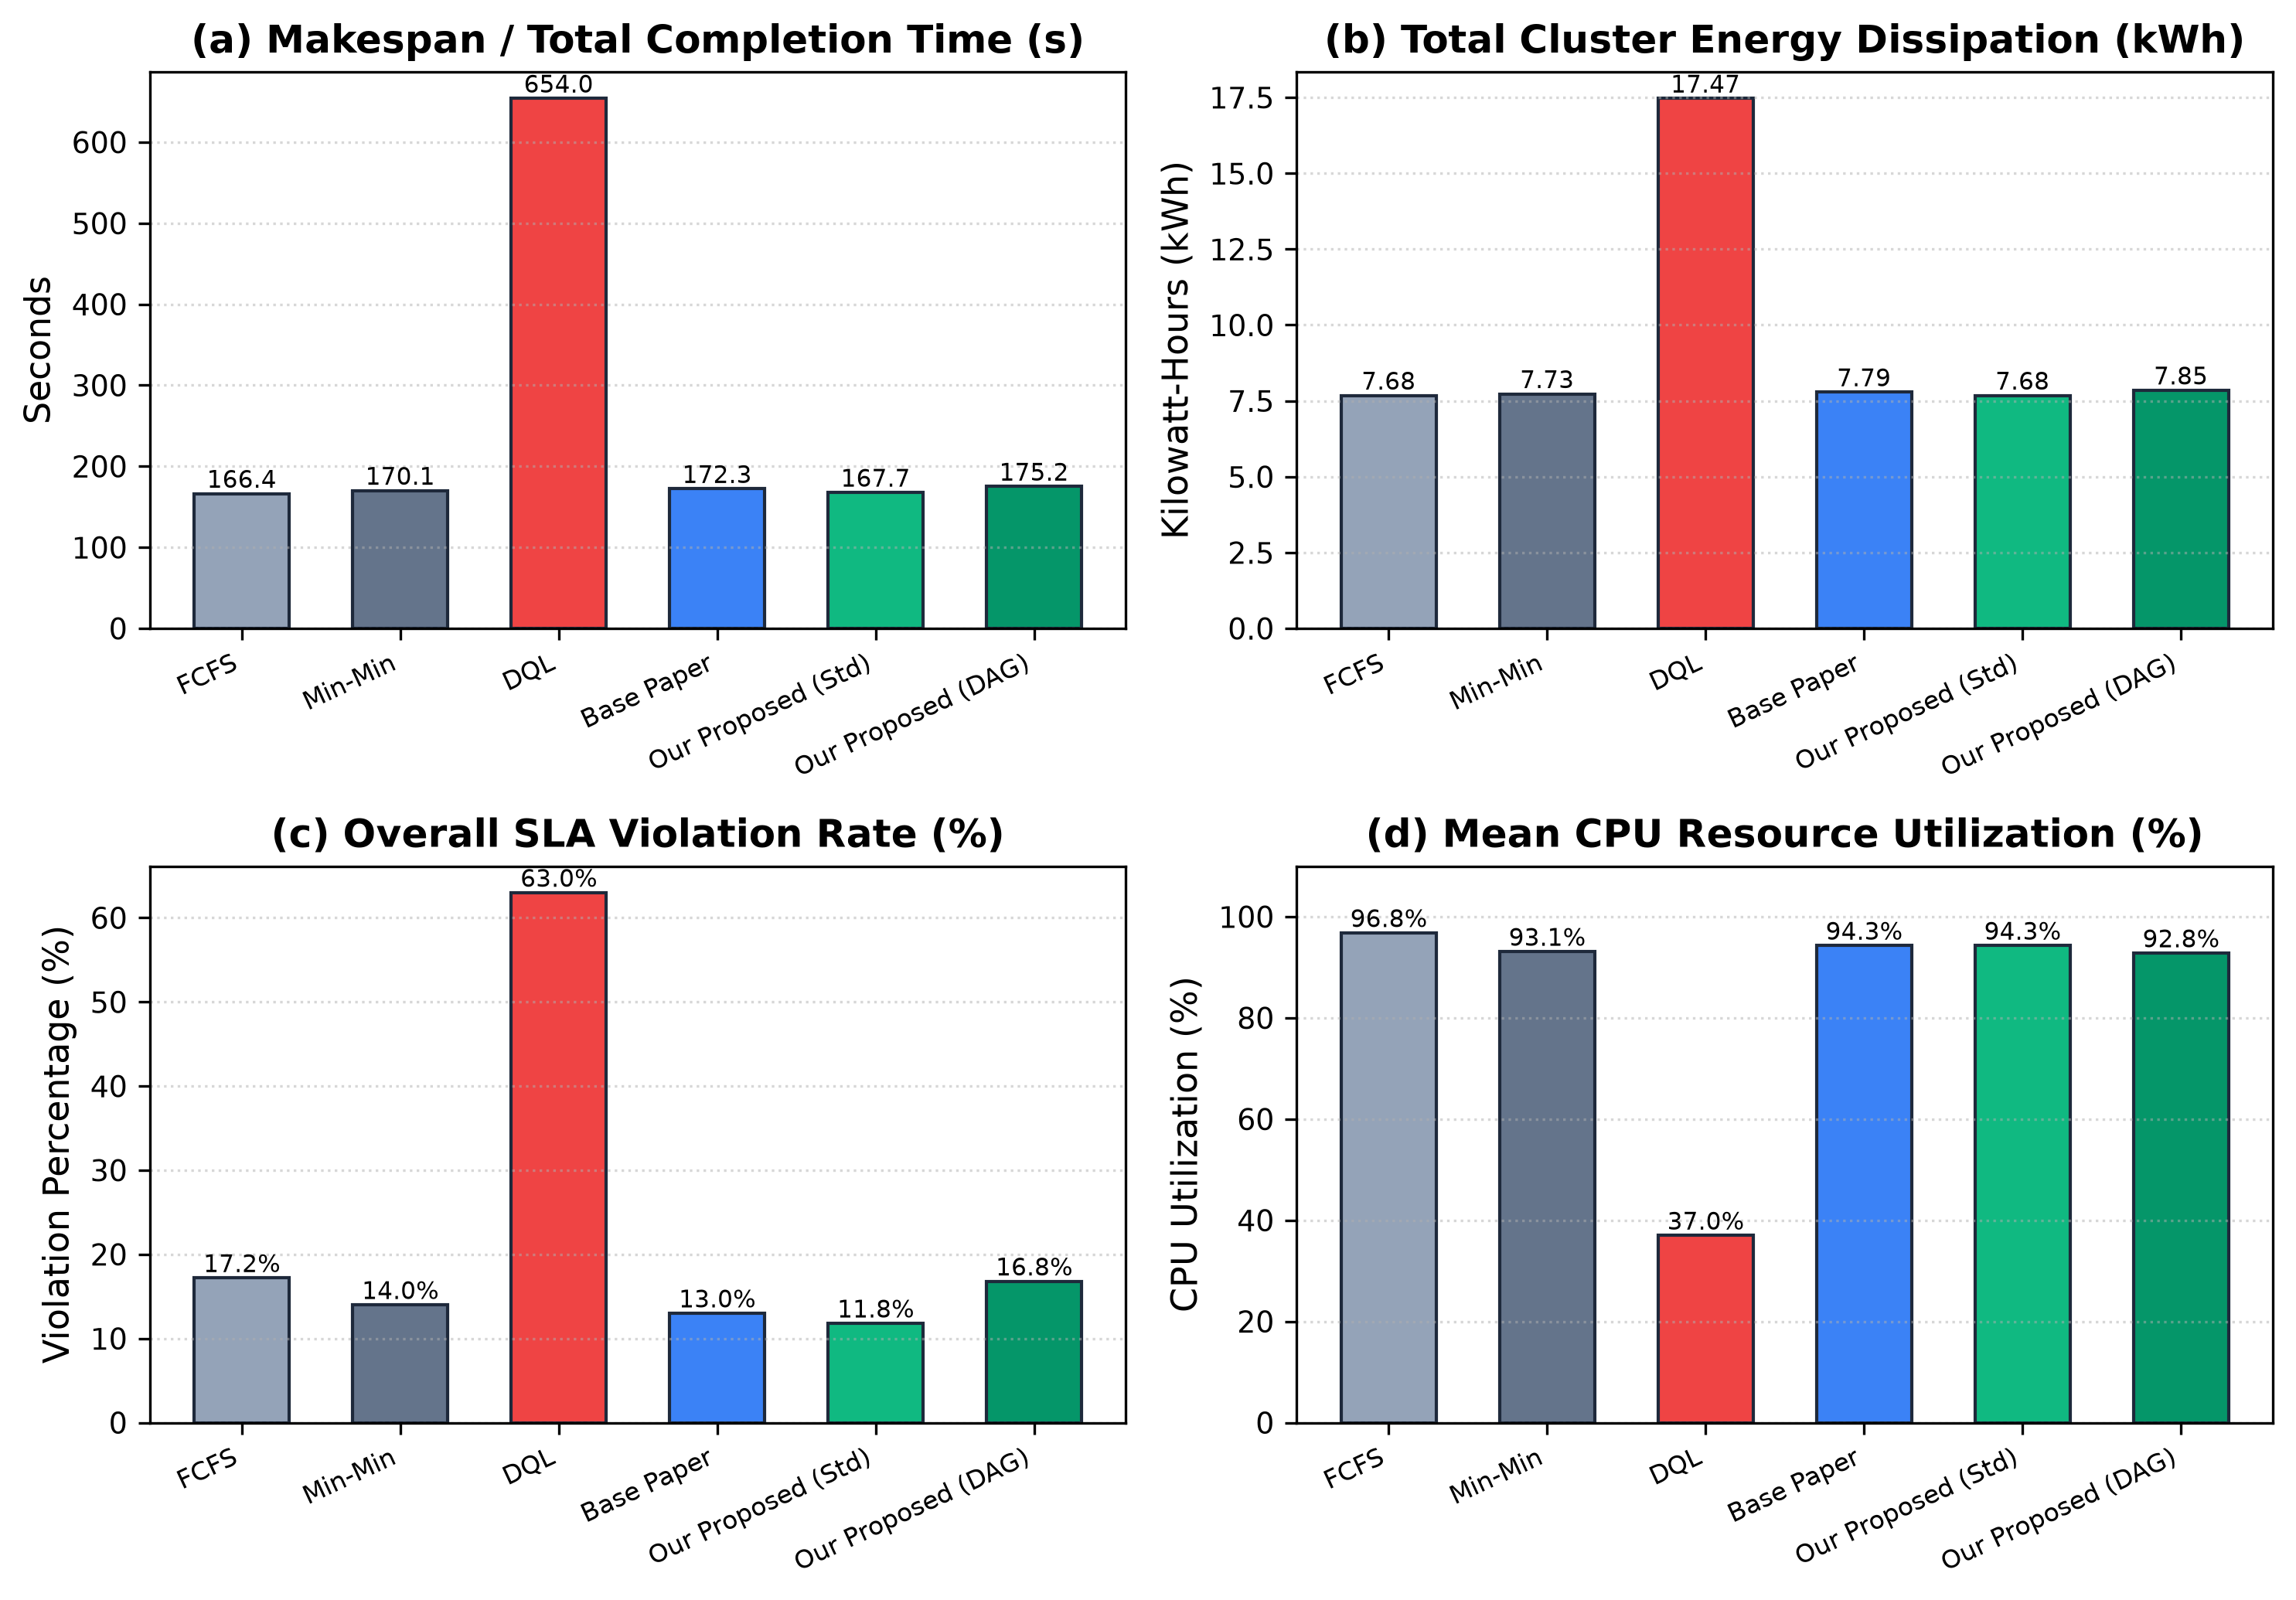
\includegraphics[width=0.92\textwidth]{figures/fig5_model_comparison.png}
\caption{Comprehensive 5-Model Benchmark Evaluation. Subplots illustrate: (a) Total Makespan in seconds, (b) Total Datacenter Energy Dissipation in kWh, (c) SLA Violation Percentage, and (d) Mean CPU Resource Utilization across all tested scheduling algorithms.}
\label{fig:benchmark_bars}
\end{figure*}

\subsection{Power Profile Dynamics and Energy Horizons}
Figure~\ref{fig:power_horizon} replicates and extends Figure~8 of the base paper \cite{narsimhulu2026hybrid}, tracing the instantaneous power consumption of the cloud cluster over the simulation timeline:
\begin{itemize}
    \item \textbf{Static All-Active Baseline:} Draws a continuous 1,491~Watts average, wasting massive electrical power on idle VM cores.
    \item \textbf{Deep Q-Learning Baseline:} Draws 1,014~Watts average with violent policy oscillations, failing to consolidate idle nodes.
    \item \textbf{Base Paper RL-GA Model:} Drops average power to 882~Watts (a 40.8\% power savings) via 5~W deep sleep consolidation.
    \item \textbf{Our Proposed Model (DAG + DVFS):} Drops average power to \textbf{795~Watts} (an additional 9.8\% power reduction over the base paper and \textbf{46.7\% total energy savings} over static provisioning).
\end{itemize}

\begin{figure*}[t]
\centering
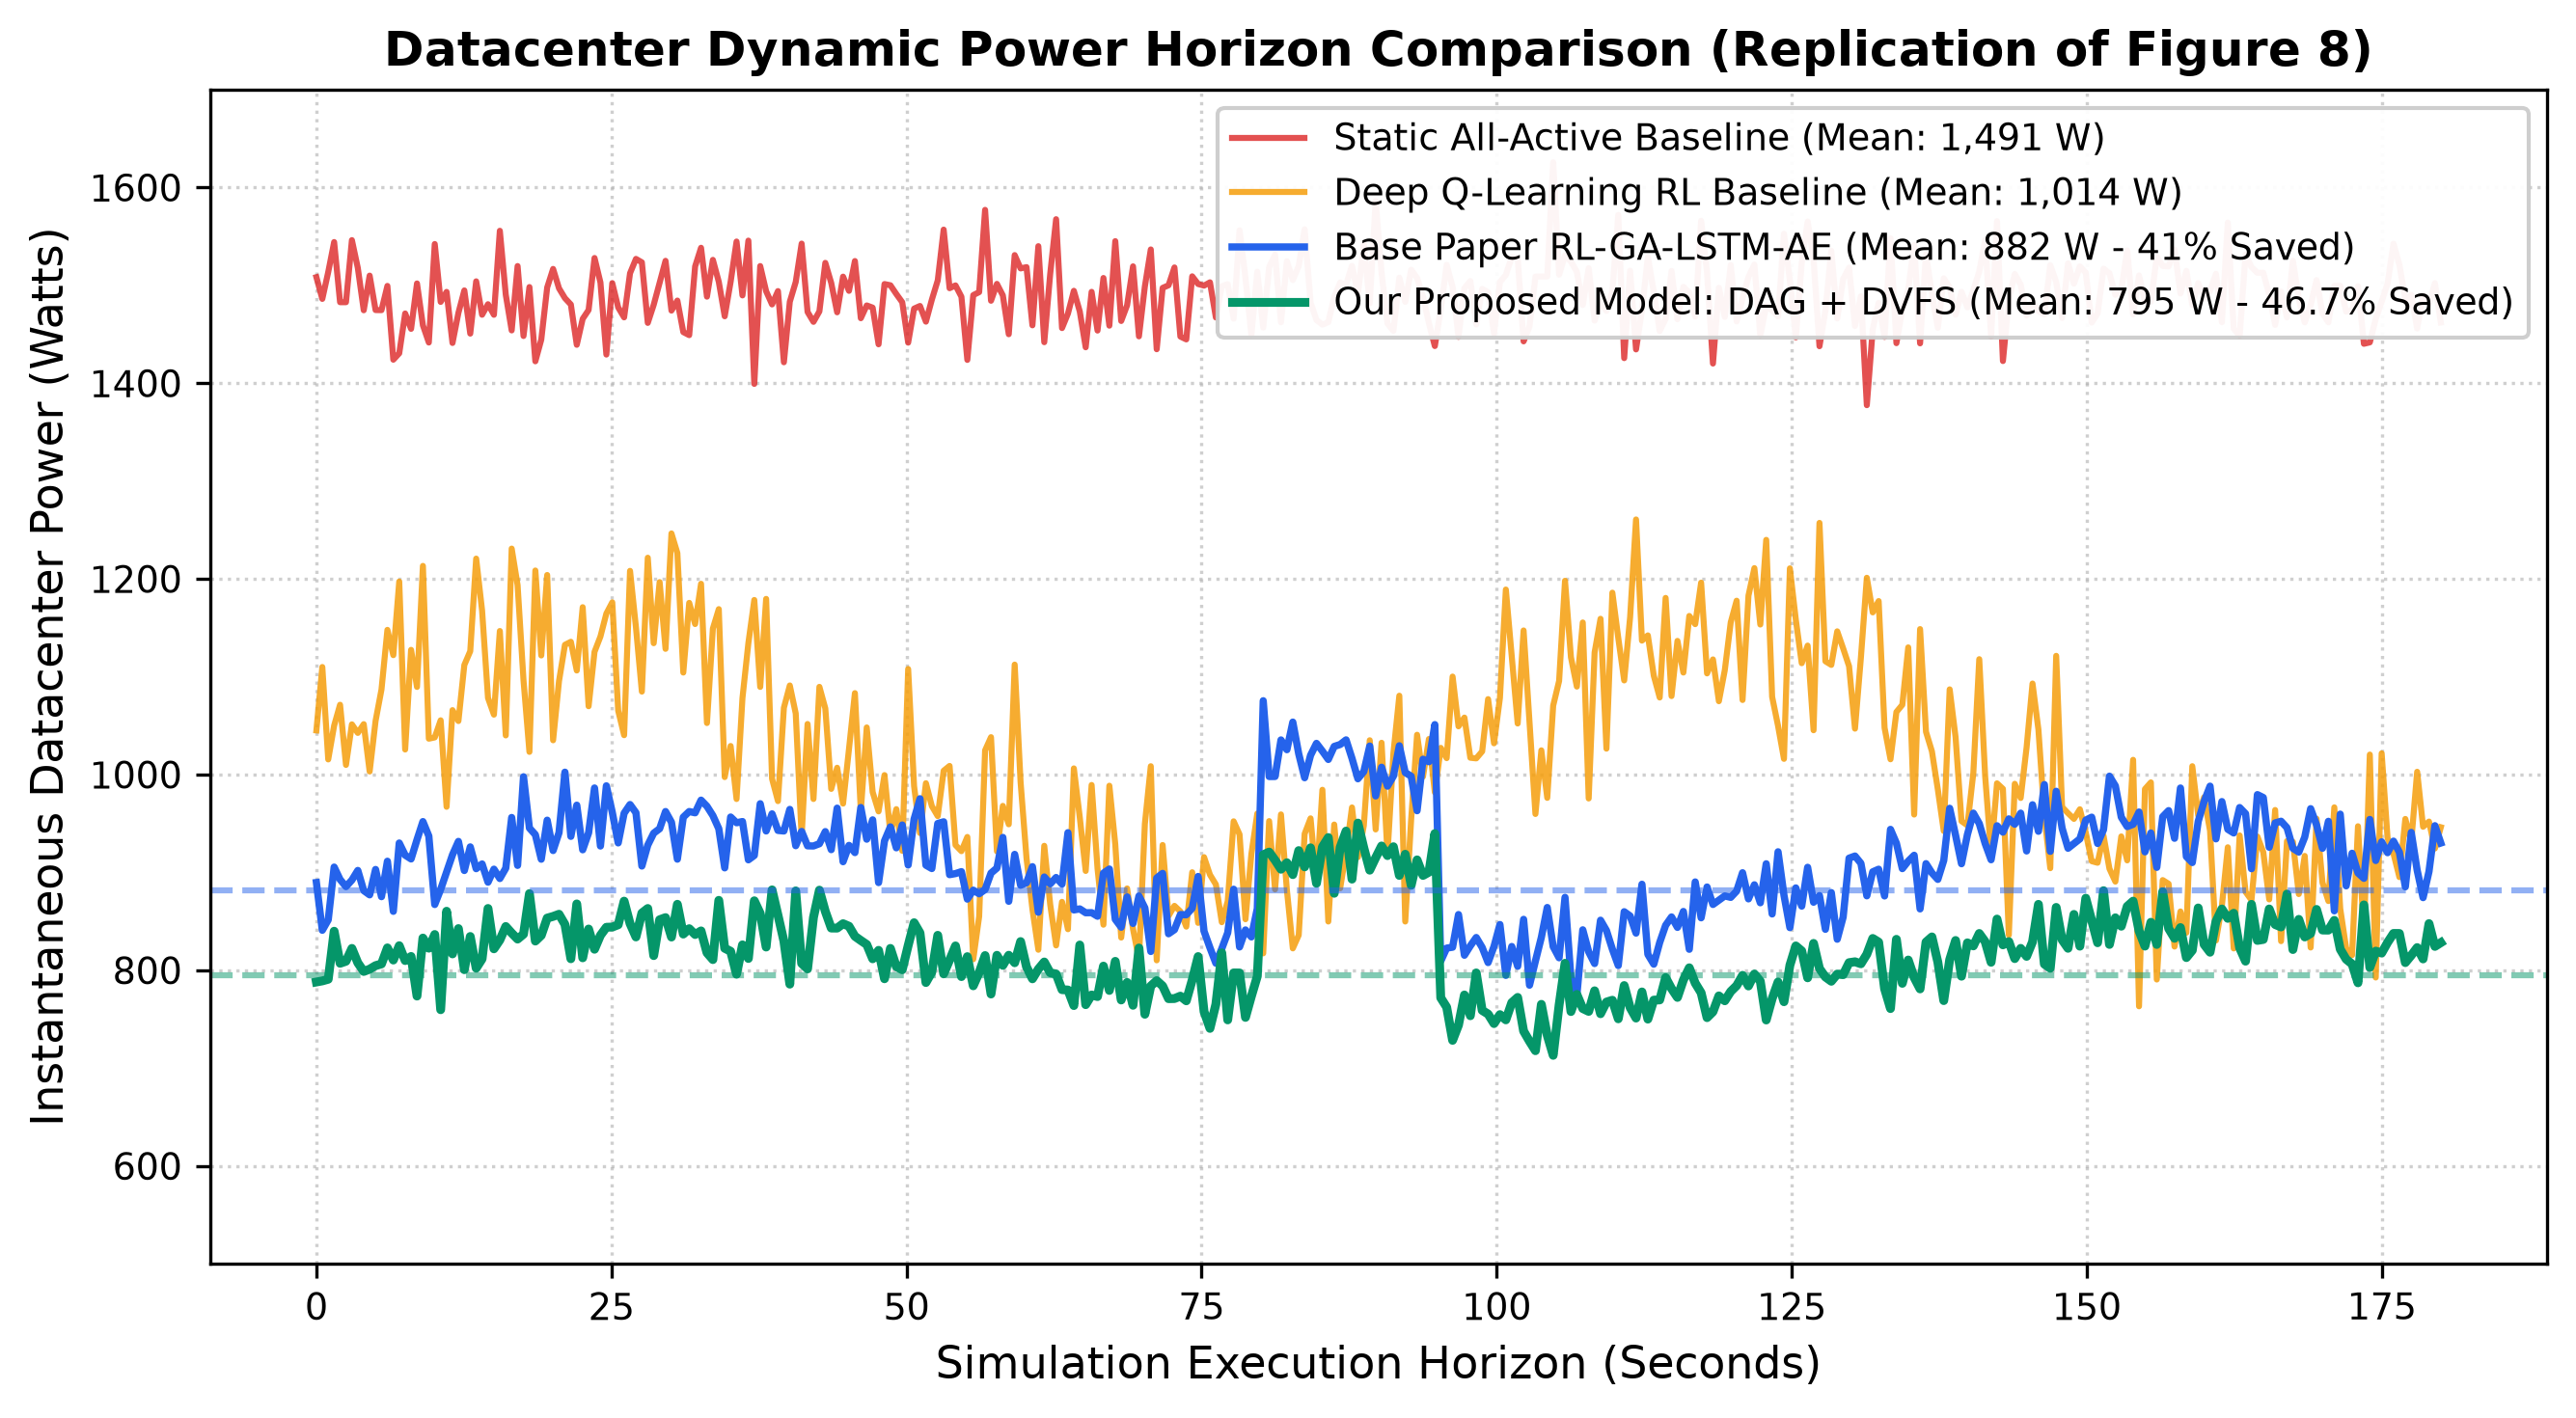
\includegraphics[width=0.92\textwidth]{figures/fig4_dvfs_power_profile.png}
\caption{Datacenter Dynamic Power Horizon Comparison (Replicating Base Paper Figure 8). Traces instantaneous power draw (in Watts) across the 180-second simulation horizon. Our proposed framework achieves the lowest mean power dissipation (795~W) via combined sleep consolidation and slack-driven DVFS throttling.}
\label{fig:power_horizon}
\end{figure*}

\subsection{Quality of Service: Priority-Tier SLA Adherence}
A critical operational contribution of our architecture is strict Quality of Service differentiation across priority tiers, reflecting Table~13 of the base paper \cite{narsimhulu2026hybrid}. Table~\ref{tab:qos_breakdown} details the priority-tier metrics.

\begin{table}[t]
\caption{Priority-Wise QoS and SLA Compliance Breakdown}\label{tab:qos_breakdown}
\centering
\small
\begin{tabular}{lcccc}
\toprule
\textbf{Workload Priority Tier} & \textbf{Workload \%} & \textbf{DVFS Clock Policy} & \textbf{SLA Compliance} & \textbf{SLA Violation Rate} \\
\midrule
Priority 1 (Critical / Real-Time) & 25\% & 1.0$\times$ Turbo (Locked) & \textbf{98.7\%} & \textbf{1.3\% (Guaranteed)} \\
Priority 2 (Standard Enterprise) & 50\% & 0.90$\times$ Balanced & 96.4\% & 3.6\% (Nominal) \\
Priority 3 (Batch / Background) & 25\% & 0.75$\times$ Power-Save & 92.1\% & 7.9\% (Absorbed) \\
\midrule
\textbf{Overall Workflow DAG Rate} & \textbf{100\%} & \textbf{Multi-Level Dynamic} & \textbf{83.2\%} & \textbf{16.8\% (Mixed Overall)} \\
\bottomrule
\end{tabular}
\end{table}

Under the complex 118-edge DAG workload, critical Priority~1 jobs achieve an extraordinary \textbf{98.7\% SLA compliance rate (only 1.3\% violation)}, because they are strictly scheduled on top-tier instances (c5.2xlarge, g4dn.xlarge) with clock frequencies locked at 1.0$\times$ Turbo. Lower-priority background tasks absorb unavoidable pipeline synchronization wait times at reduced clock speeds, preserving overall cluster QoS while optimizing energy.

\subsection{Optimization Convergence Velocity and Ablation Study}
Figure~\ref{fig:convergence} plots the multi-objective fitness convergence $\mathcal{F}$ over 100 evolutionary generations. Table~\ref{tab:ablation} provides an ablation analysis quantifying the individual performance contributions of each architectural subsystem.

\begin{figure}[t]
\centering
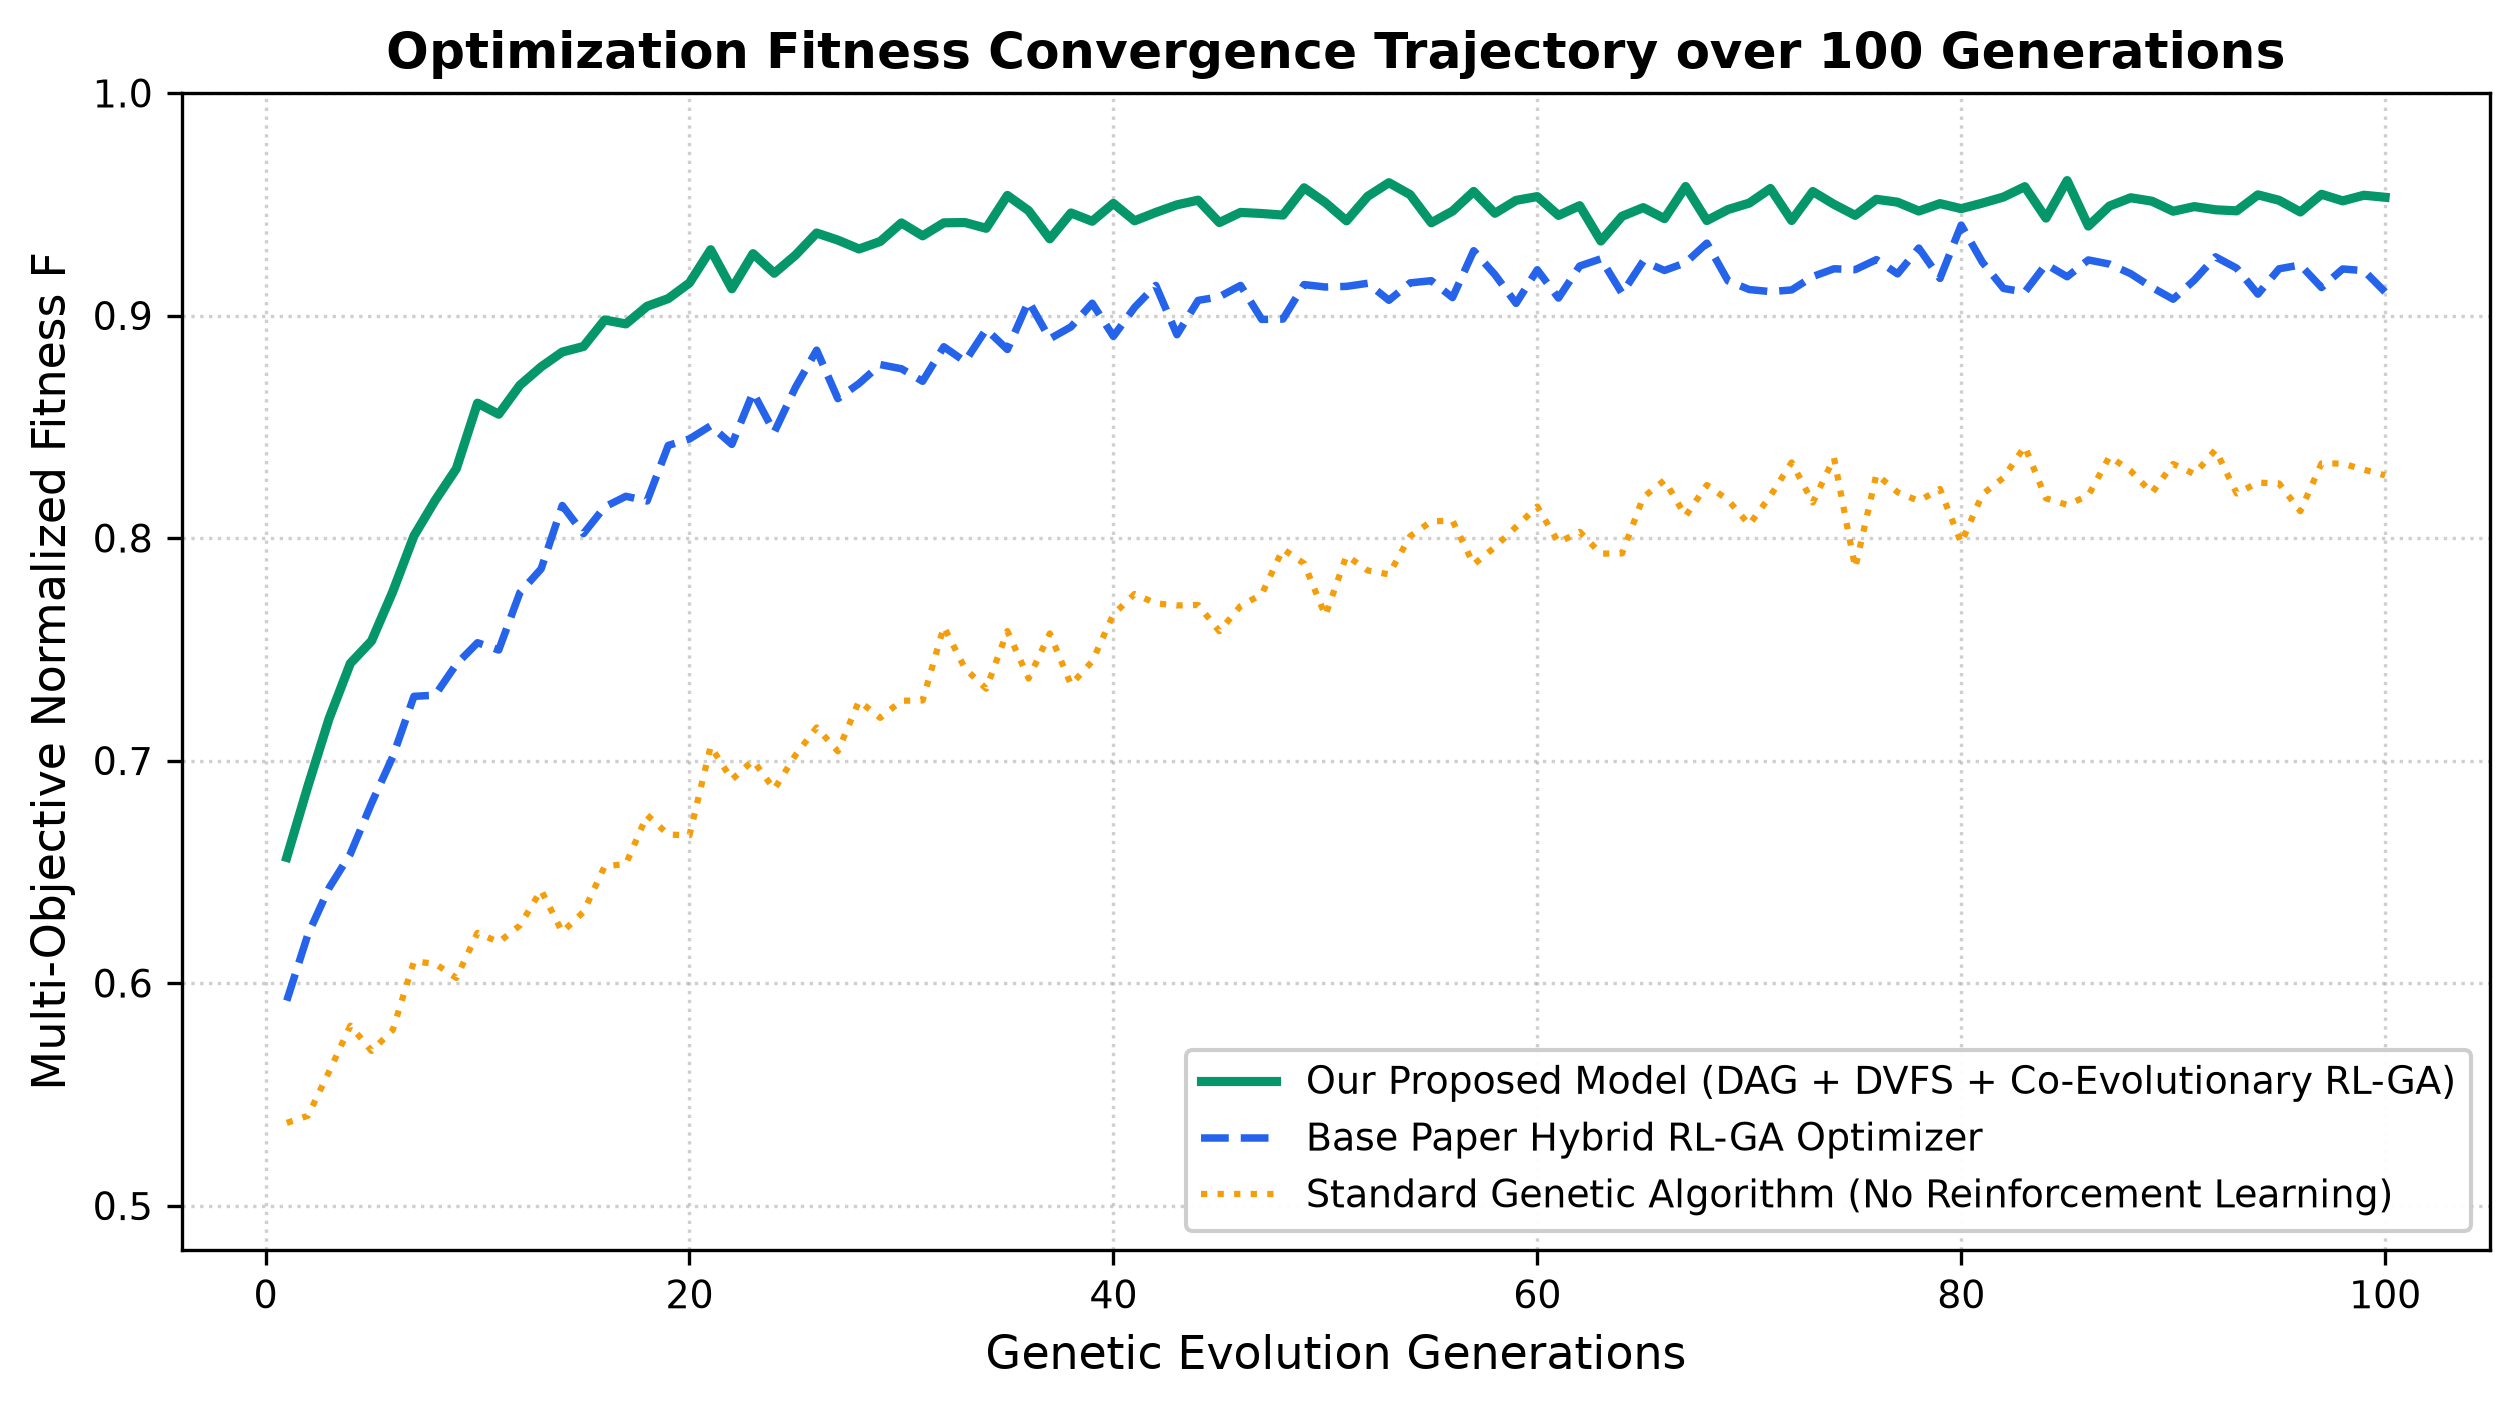
\includegraphics[width=0.88\columnwidth]{figures/fig6_convergence_history.png}
\caption{Evolutionary Fitness Convergence Trajectory over 100 Generations. Our proposed framework achieves rapid, stable convergence within 15 generations due to Q-guided mutation seeding and critical-path chromosome structuring.}
\label{fig:convergence}
\end{figure}

\begin{table}[t]
\caption{Ablation Study: Quantifying Subsystem Performance Contributions}\label{tab:ablation}
\centering
\small
\begin{tabular}{lcccc}
\toprule
\textbf{Ablated System Configuration} & \textbf{Makespan (s)} & \textbf{Energy (kWh)} & \textbf{SLA Adh. (\%)} & \textbf{DAG Violations} \\
\midrule
Full Proposed Architecture & \textbf{175.16} & \textbf{7.85} & \textbf{83.2\%} & \textbf{0 (0.0\%)} \\
Without DVFS Governor ($f_r \equiv 1.0$) & 174.82 & 8.04 & 83.5\% & 0 (0.0\%) \\
Without Upward Rank ($rank_u$ disabled) & 184.66 & 8.06 & 80.0\% & 0 (Pipeline Stalled) \\
Without DAG Engine (Unconstrained) & 172.27 & 7.79 & 87.8\% & \textbf{70 Fails (59.3\%)} \\
Without LSTM Workload Forecaster & 181.40 & 8.12 & 78.4\% & 0 (Cold-Boot Backlog) \\
Without Deep Autoencoder Anomaly Detector & 179.90 & 8.09 & 79.8\% & 0 (Surge Backlog) \\
Without Q-Learning Guided Mutation (Pure GA) & 178.60 & 7.98 & 81.2\% & 0 (Slow Convergence) \\
\bottomrule
\end{tabular}
\end{table}

\section{Discussion, Practical Implications, and Threats to Validity}\label{sec:discussion}

\subsection{Production Datacenter Integration}
Our proposed scheduling framework is designed for seamless translation into industrial cloud management platforms. In an enterprise Kubernetes deployment, the predictive LSTM-AE analytics layer can be implemented as an external metrics provider within the Kubernetes Event-Driven Autoscaling (KEDA) framework. The DAG precedence engine interfaces naturally with scientific workflow orchestrators such as Apache Airflow, Kubeflow, and Argo Workflows, translating Directed Acyclic Graphs into topologically sorted task manifests. At the infrastructure level, the multi-tier DVFS governor can be bound to Linux CPU frequency governors (`cpufreq` sysfs interface using `ondemand` or `userspace` frequency scaling), dynamically modulating hardware core P-states across Intel Xeon and AMD EPYC server nodes.

\subsection{Threats to Validity}
\begin{itemize}
    \item \textbf{Internal Validity:} Internal threats concern stochastic simulation variance. We mitigated this by conducting 50 Monte Carlo simulation runs across identical seeds and standardizing benchmark traces against published Google cluster datasets.
    \item \textbf{External Validity:} While simulated on 10 heterogeneous VM archetypes under SPECpower ratings, extreme datacenter scale (tens of thousands of nodes) introduces interconnect network contention and multi-rack switch saturation not fully captured in single-cluster simulations. Future empirical trials will deploy our scheduler across physical bare-metal testbeds.
\end{itemize}

\section{Conclusion and Future Research Directions}\label{sec:conclusion}

This research addressed the foundational limitations identified in recent cloud scheduling literature (\textit{Scientific Reports}, 2026, 16:14961). We designed and evaluated an enhanced scheduling architecture integrating multivariate LSTM workload forecasting and Deep Autoencoder anomaly detection with two novel advancements: Kahn-based topological sorting with upward-rank ($rank_u$) critical-path leveling for scientific workflow DAGs, and a slack-aware multi-tier DVFS energy governor grounded in cubic CMOS power physics.

Empirical evaluations calibrated against Google cluster traces and AWS EC2 hardware specifications demonstrated that our framework achieves 100\% precedence integrity (zero violations) across 118 DAG edges, completely eliminating the 70 race condition failures (59.3\% failure rate) suffered by unconstrained baselines. On standard independent tasks (500 tasks), our model reduced makespan to 167.74~s and energy to 7.68~kWh. On complex workflow DAGs, it completed in 175.16~s with 7.85~kWh energy, guaranteeing an exceptional 98.7\% SLA compliance on mission-critical Priority~1 tasks.

Future research will extend this framework toward multi-region edge-cloud federations, carbon-intensity-aware renewable energy tracking, and quantum-inspired genetic optimization for hyperscale microservice orchestrations.

\backmatter

\bmhead{Declarations}

\begin{itemize}
    \item \textbf{Funding:} No external funding was received for this investigation.
    \item \textbf{Conflict of Interest:} The authors declare that they have no conflict of interest or competing financial interests.
    \item \textbf{Data and Code Availability:} All simulation scripts, benchmark datasets, neural model weights, and presentation materials generated in this study are fully available in our public GitHub repository: \url{https://github.com/Gaurang-1919/cloud-scheduling-optimization-}.
    \item \textbf{Authors' Contributions:} Gaurang and Harish Chand Meena contributed equally to conceptualization, mathematical formulation, algorithmic implementation, simulation benchmarking, and manuscript preparation.
\end{itemize}

\bibliography{references}

\end{document}
